%!TEX program = xelatex
\documentclass[11pt,article,oneside]{memoir}
\usepackage{org-preamble-xelatex}
\DisemulatePackage{setspace}
\usepackage{setspace}
\usepackage{titling}
\setlength{\droptitle}{-12em}
% \input{vc}


\usepackage{graphicx}
% We will generate all images so they have a width \maxwidth. This means
% that they will get their normal width if they fit onto the page, but
% are scaled down if they would overflow the margins.
\makeatletter
\def\maxwidth{\ifdim\Gin@nat@width>\linewidth\linewidth
\else\Gin@nat@width\fi}
\makeatother
\let\Oldincludegraphics\includegraphics
\renewcommand{\includegraphics}[1]{\Oldincludegraphics[width=\maxwidth]{#1}}


%\author{}

\author{}

%\author{}

\date{}


\begin{document}  
\setkeys{Gin}{width=1\textwidth} 	
\setromanfont[Mapping=tex-text,Numbers=OldStyle]{Georgia} 
\setsansfont[Mapping=tex-text]{Gill Sans} 
\setmonofont[Mapping=tex-text,Scale=0.8]{Consolas}
\chapterstyle{article-jmrphy}
\pagestyle{kjh}

\singlespacing





\thispagestyle{empty}

\section{Mass Media and Civil War
Onset}\label{mass-media-and-civil-war-onset}

Justin Murphy \newline
University of Southampton \newline     
Department of Politics and International Relations \newline     
\href{mailto:j.murphy@soton.ac.uk}{j.murphy@soton.ac.uk} \newline    

\paragraph{Abstract:}\label{abstract}

Qualitative evidence suggests that mass media can play a causal role in
the outbreak of civil war and, at the international level, the rapid
increase of mass media in recent decades has coincided with a similarly
notable surge in civil war prevalence. Yet recent quantitative research
suggests that mass media decrease the probability of civil war onset by
enhancing the power of states and therefore deterring insurgencies. To
explain this puzzling contradiction, I argue that mass media
technologies have a non-linear effect on the probability of civil war
onset. Mass media technologies should decrease the likelihood of civil
war onset only above the threshold at which they constitute a mass
communications system. Below that threshold, increases in mass media
should increase the likelihood of civil war. The theory is tested with
parametric and semi-parametric regressions on country-level,
cross-sectional time-series data from a recent study (Warren 2014) and
long-run historical time-series at the international level. I find
evidence of substantial non-linearity in the effect of mass media on
civil war onset at both levels of analysis. This research note
contributes an important new insight into the causes of civil war and
contributes to the burgeoning research agenda on the nexus of
information-communication technology (ICT) and political
conflict.\newline

Last updated: January 29, 2015.\footnote{This is a draft working paper.
  Comments, questions, and suggestions are welcome and can be emailed to
  \href{mailto:j.murphy@soton.ac.uk}{j.murphy@soton.ac.uk}. If you wish
  to cite, please use
  \href{http://figshare.com/authors/Justin_Murphy/498998}{the citation
  with DOI provided by Figshare}, though please check back for future
  updates.} \newline

\clearpage
\pagenumbering{arabic}

\onehalfspacing

Current research on the relationship between mass media and civil war
onset is puzzling. From Rwanda and Yugoslavia in the early 1990s to
Libya and Syria in 2011, civil wars often involve the use of mass media
for belligerent purposes (Hubbard and Saad 2014; Kirkpatrick 2011;
``Roads Sealed as Yugoslav Unrest Mounts'' 1990; Simons 2002). While
some scholars argue that mass media play a causal role in the outbreak
of civil wars (Brass 1997; Des Forges 1999; Gagnon Jr 1994; Kellow and
Steeves 1998; Metzl 1997; Tambiah 1996), others have argued that the
negative effects of mass media have been overstated (Paluck 2009; Straus
2007). Making the puzzle even more acute, the most systematic evidence
to date suggests that mass media induce satisfaction with the status quo
(Kern and Hainmueller 2009) and decrease the likelihood of civil war
onset (Warren 2014). Yet, as Figure 1 illustrates, at the global level
the exponential increase in mass media beginning in the 1950s coincides
with a similarly dramatic increase in civil wars at the global
level.\footnote{For a description of the variables see Data and Method
  below.} If mass media decrease the probability of civil war, it is
puzzling that the proliferation of mass media since the 1950s coincides
with a surge in civil war prevalence beginning in the 1960s.

\begin{figure}[htbp]
\centering
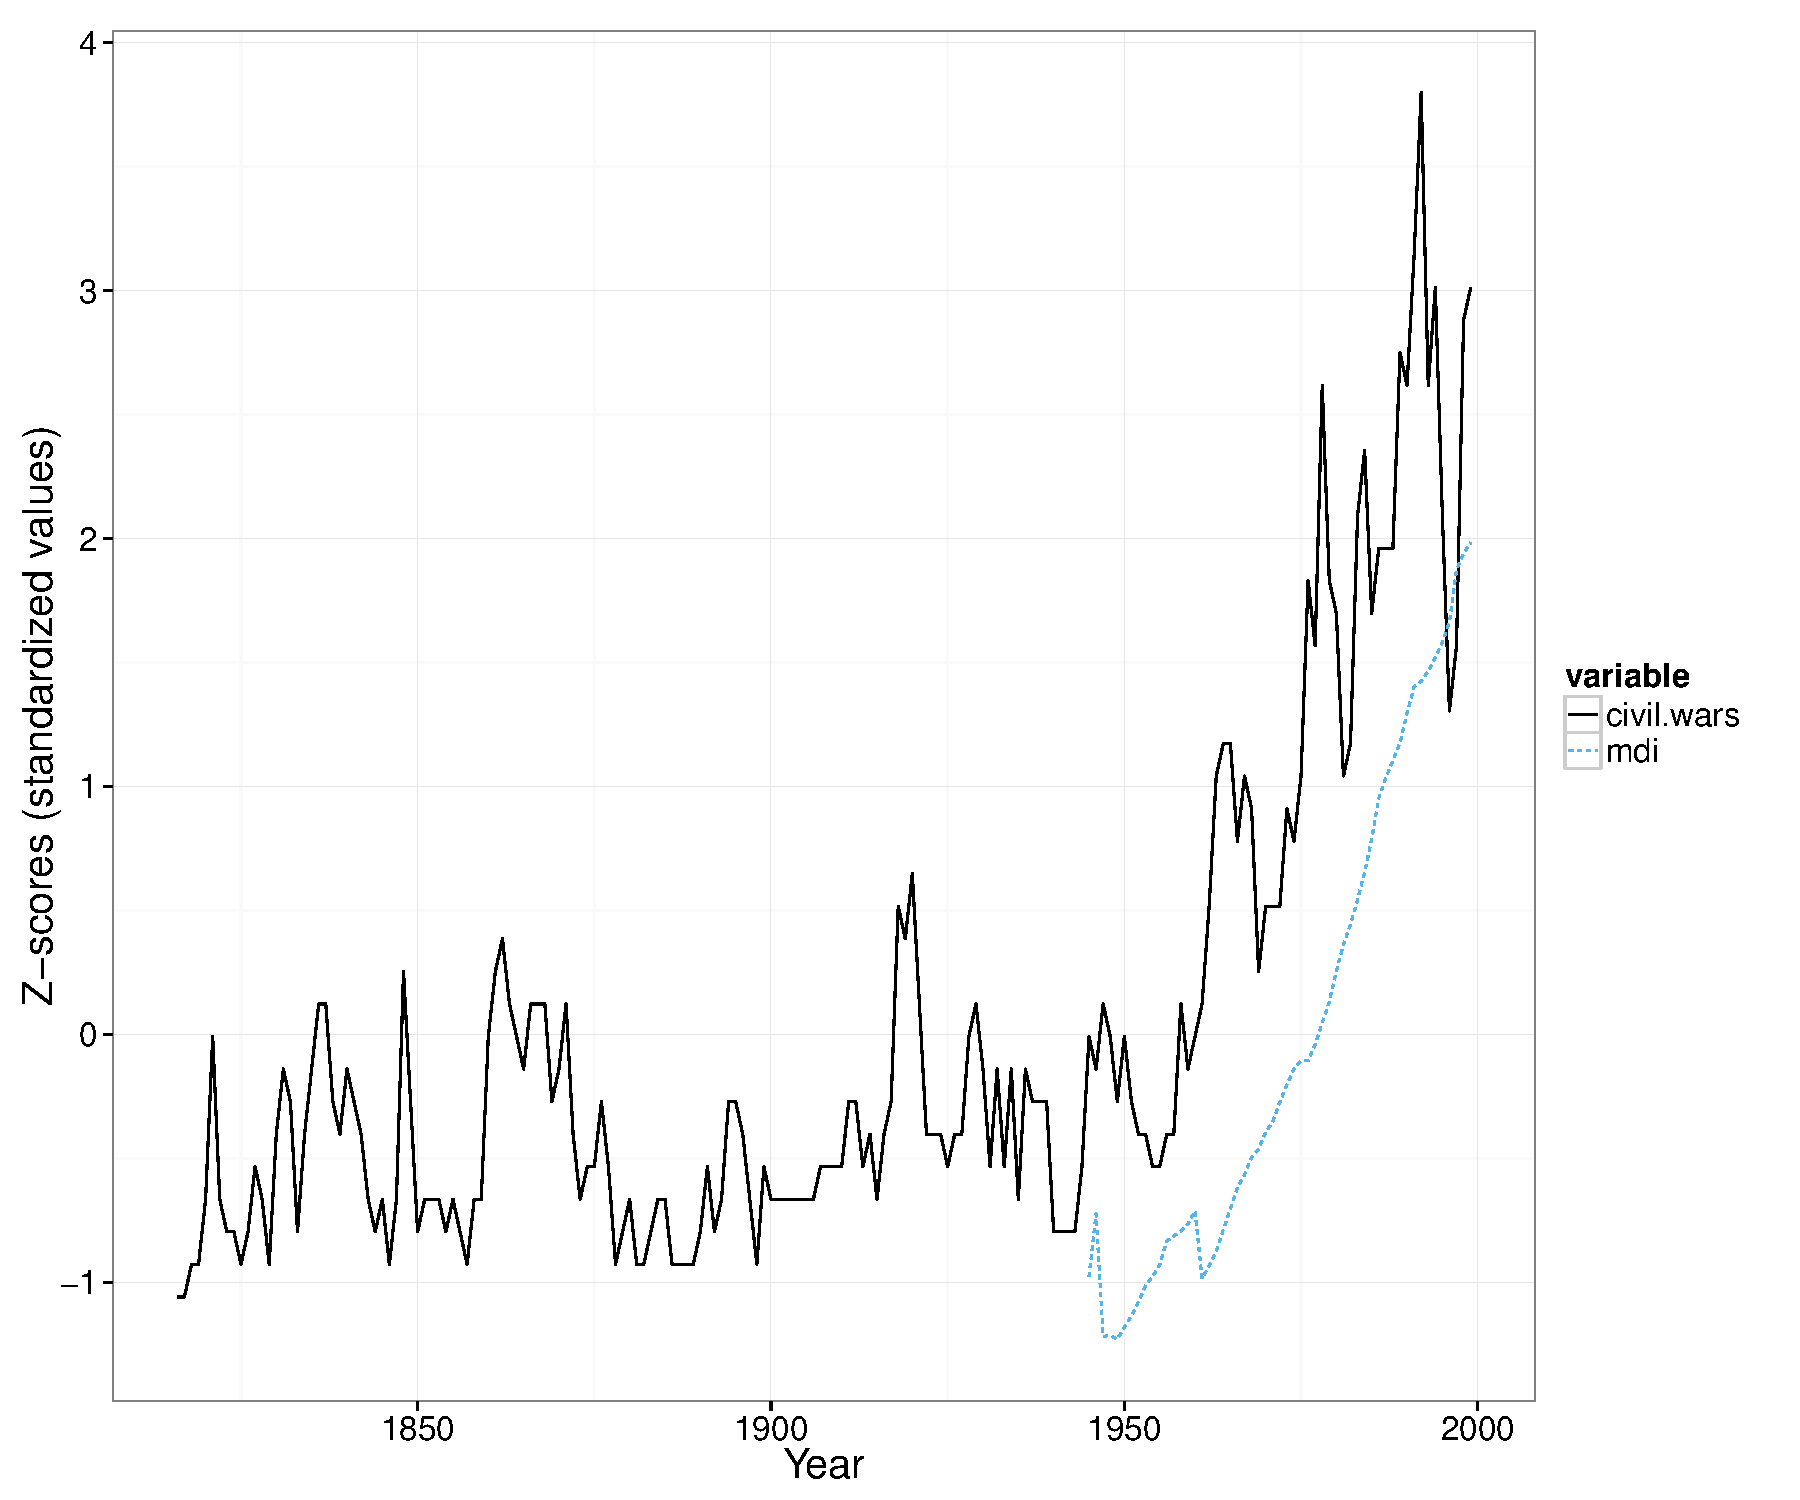
\includegraphics{media_civil_war_files/figure-markdown/globalplot.pdf}
\caption{Mass Media Density and Civil Wars Globally, 1816-1999}
\end{figure}

This research note advances a novel theoretical proposition on the
relationship between mass media and civil war which accounts for
previous qualitative findings of mass media fomenting civil war onset as
well as recent quantitative evidence that mass media decrease the
probability of civil war onset. Paradoxically, it is precisely because
dense mass media systems strengthen the state that the first appearance
and early spread of mass media within a country should \emph{encourage}
insurgencies. When mass media spreads enough within a country to
constitute a mass communications system, this triggers communicative
economies of scale which so increase the payoffs of controlling the
state that it incentivizes violent insurgency before the \emph{ex ante}
holders of state power become normatively locked-in and effectively
impossible to challenge.\footnote{As discussed below, beyond a certain
  threshold of mass media the probability of observing a civil war is
  effectively zero.} A key point of my account, however, is that the
economies of scale peculiar to information production within a mass
communications system represent a qualitative change which occurs only
when the spread of mass media crosses a certain threshold. This is why
there is an inflection point at which the effect of mass media should
change from positive to negative beyond a certain level of mass media
density. The counter-intuitive implication is that the very pacifying
effect of a mass communications system charges the early spread of mass
media with a bellicose effect until the threshold of mass communications
is crossed.

To compare the non-linear, war-before-peace theory to the linear,
general pacification theory, I generate causal leverage by deducing two
new observable implications at two levels of analysis, within and
outside the original sample used in the most recent and systematic study
on this question (Warren 2014). I use a combination of parametric and
semi-parametric regressions to compare linear and non-linear model fits
on the original sample. I then consider long-term historical time-series
at the international level, to examine whether the war-before-peace
theory helps explain the empirical pattern of civil war prevalence at
the international level.

The implications of this research note are twofold. First, this research
note contributes to the project of building ``rich theory'' for the new
and burgeoning research agenda on the ICT and political conflict nexus
(Lyall and Dafoe 2015), demonstrating in particular the importance of
non-linearities in this area.\footnote{Lyall and Dafoe advocate that
  research on the ICT and political conflict nexus should be
  increasingly ``elaborate,'' focusing on the highly conditional effects
  of ICT, developing theories grounded in well-established findings, and
  tested for multiple observable implications. In particular, they
  highlight that for some causal processes, ``Effects may not arise
  until some culminating point is reached,'' and they ``may change in
  sign over time, as actors strategically adapt to their new information
  environment'' (Lyall and Dafoe 2015, 3--4).} Second, it contributes
novel quantitative evidence helping to explain the severity and timing
of one of the most lethal dynamics in the world since World War II: the
increase in civil wars around the world beginning in the 1950s and 1960s
(Fearon and Laitin 2003, 75).

This research note proceeds as follows. The first section provides a
brief summary and critique of the general pacification theory, providing
the basic rationale for why we should expect the relationship between
mass media and civil war onset to be non-linear. The second section
states the non-linear, war-before-peace theory and deduces two
observable implications which are mutually exclusive with the general
pacification theory. The third section explains the data sources,
variables, and modeling strategy. A fourth section discusses the results
and a fifth section concludes.

\section{A Critique of the General Pacification Theory of Mass Media and
Civil
War}\label{a-critique-of-the-general-pacification-theory-of-mass-media-and-civil-war}

Many scholars of the modern nation-state have argued that by allowing
political elites to communicate with subjects across large territories,
the emergence of mass media technologies was a crucial condition for the
emergence of the modern nation-state (Anderson 1983; Deutsch 1953).
Within this tradition, contemporary political scientists often
conceptualize mass media technologies as instruments which increase the
state's ``soft power'' to induce loyalty and symbolic attachments
(Keohane and Nye 1998; Nye 1990, 168--69, 2004, 47--48). Issuing from
this perspective, one recent article argues that by increasing the
state's communicative power, mass media deter potential insurgencies and
therefore decrease the probability of civil war onset (Warren 2014).

According to Warren, technologies such as televisions, radios, and
newspapers decrease the probability of civil war onset because they
increase the state's communicative power more than the communicative
power of potential challengers. While mass media technologies lower the
costs of communication for the state and potential challengers alike,
mass media technologies increase the normative influence of the state in
particular because of economies of scale which are unique to the
production of normative influence. Because a media message achieves a
larger effect on receivers who believe the message was widely
disseminated, the production of normative influence through mass media
brings increasing marginal returns for each additional unit of effort,
as each additional recipient receiving the message increases the effect
of the message on the rest of the receivers. Because the state is
inherently a larger-scale producer of symbolic content than potential
insurgent groups, higher levels of mass media are expected to make
stronger states and therefore lower the probability of observing civil
war.

Using state-level data for a large panel of countries from 1945 to 1999,
Warren constructs a media density index (MDI) on a country-year basis
capturing the total number of televisions, radios, and newspapers per
100 people.\footnote{The measure is discussed in greater detail below.}
Warren demonstrates that, after controlling for other predictors of
civil war, mass media density is associated with more than a tenfold
decrease in the likelihood of observing civil war in a particular
country-year.

The general pacification theory has two key logical shortcomings. First,
the unique logic of mass communications which is expected to benefit the
state's inclusive national appeals more than insurgents' divisive
appeals should not be linearly increasing with mass media density but
should rather be contingent on a certain threshold of mass media
density. To the degree mass media simply lower the costs of
communication, they empower insurgents no less than the state (Warren
2014, 120). The crucial reason why mass media disproportionately amplify
the normative influence of the state (why there are increasing marginal
returns to the production of influence) is that receivers believe the
message is widely spread (Chwe 1998, 2001; Mutz 1998), that mass media
messaging is ``known by all to have been seen by all'' (Warren 2014,
120). The key point is that at very low levels of mass media density
there is no reason one receiver of a message should be impressed by a
very small number of others who may have received the message. Only
after a certain threshold or ``tipping point,'' at which a ``critical
mass'' of receivers are expected to receive mass media messaging, should
there be increasing marginal returns to the production of influence.
National situations in this post-threshold situation I refer to as
``mass communications systems.'' National situations below this
threshold I refer to as ``pre-mass communications systems.''

Increases in mass media density only uniquely benefit the state's
production of influence and therefore decrease the likelihood of civil
war beyond the threshold at which mass media technologies are
sufficiently widespread to effectively consititute a mass communications
system.\footnote{I assume throughout that mass media typically first
  appears within countries at very low levels relative to the population
  (low media density). I also assume throughout that, despite variable
  rates of change and short-run decreases, media density has a long-run
  tendency to increase. In other words, I assume that the dynamics of
  media density are non-stationary and trend upward. The Levin-Lin-Chu
  (2002) and Im-Pesaran-Shin (2003) tests for stationarity in panel data
  fail to reject the null hypothesis that media density is
  non-stationary (p = 0.7473 and p = 0.1, respectively). See
  Supplementary Information for details.} When only a very small
proportion of the population has access to mass media technologies,
those technologies do not imply the presence of a mass communications
system at merely low levels; they imply a country which still
categorically lacks the infrastructural capacity for properly mass
communications.\footnote{There is no way to know \emph{a priori} how
  many people need access to mass media technologies before they
  constitute a mass public network and therefore the categorical
  presence of a mass communications system. The question is pursued
  empirically below.}

Second, if the level of mass media increases state strength, then the
\emph{first appearance and early growth} of mass media within a country
should increase the utility of controlling the state relative to other
means of influencing it. The first appearance of mass media technology
should increase the incentives of opposition groups to risk insurgency
before the development of a mass communications system significantly
increases the power of the incumbent and decreaes the power of
opposition groups outside the state. The closer a country's mass media
density is to the threshold at which it will constitute a capacity for
mass communications, the more attractive it will be for opposition
groups outside the state to gain control of the state. It is
increasingly urgent as the state becomes nearer to consolidating its
normative power via mass communications and therefore significantly less
vulnerable to insurgency; also, the closer a country is to the threshold
the less time will a successful insurgency be vulnerable to yet another
insurgency before its own normative power is consolidated by a mass
communications system. Thus, if it is true that increasing mass media
density makes state power increasingly safe from insurgency, then before
media density crosses the threshold of constituting mass communications
power, each increase in mass media density should further increase the
payoffs to violent insurgency.

\section{A Non-Linear Theory of Mass Media and Civil
War}\label{a-non-linear-theory-of-mass-media-and-civil-war}

This section advances a modified theory of the relationship between mass
media technology and civil war: while high levels of mass media density
should indeed decrease the likelihood of civil war by increasing state
power and deterring insurgents, for this very reason the
\emph{introduction and early growth} of mass media density within a
country should \emph{increase} rather than decrease the likelihood of
civil war. Precisely because a capacity for mass communications
increases state power and becomes a robust deterrent against insurgents,
but low levels of mass media density do not yet constitute that power,
year-to-year increases in mass media density up to a certain threshold
should be positively associated with civil war onset. It is only beyond
that threshold that a negative relationship between mass media density
and civil war should hold.

To test whether this modified theory is preferable to the original,
general pacification theory, I deduce two distinct observable
implications which are mutually exclusive with the original theory,
increasing causal leverage by exposing the new, modified theory to new
opportunities for falsification (Ging King, Keohane, and Verba 1994,
30). If the modified, non-linear theory is correct, then each of the
following should be true:

\textbf{Hypothesis 1:} There should exist a threshold of mass media
density below which year-to-year increases in mass media density
\emph{increase} the probability of civil war. This implication flows
directly from the logical critique of the original theory: If a system
of mass communications constitutes a significant increase in the soft
power of states and makes insurgency significantly more difficult, then
every increase in mass media density (the dynamics of which are
non-stationary and upward-trending) incentivizes insurgency without yet
increasing the risks.

\textbf{Hypothesis 2:} Given that mass media density increased markedly
after World War II from near-zero levels as measured at the
international level, year-to-year increases in mass media density at the
international level should be associated with increases in the quantity
of civil wars at the international level. On the contrary, if the
general pacification theory is correct, then year-to-year increases in
media density around the world should be associated with a decrease in
civil war onsets, controlling for other determinants of civil war onset.
Note, however, that the war-before-peace theory is consistent with the
general pacification theory in the expectation that mass media density
in the long run has a pacifying effect on the likelihood of civil war
onset, after controlling for the bellicose implications of year-to-year
changes.

\section{Data and Method}\label{data-and-method}

The first investigation for H1 uses the replication data from Warren
(2014), a panel dataset of country-level variables covering 175
countries over a maximum of 55 years in the period 1945-1999. As the
variables used in the present analyses follow the original analyses as
closely as possible, for the sake of consistency and comparison, readers
may consult the original article for a more detailed discussion of the
data. Briefly, the dependent variable in all analyses is \emph{CIVIL WAR
ONSET}, which takes a value of 1 for all country-years in which a civil
war begins and zero otherwise. Civil wars are defined, following
Sambanis (2004), as any armed challenge to state sovereignty with
explicit political objectives, local recruits, and more than 500 deaths
in the first year or more than 1,000 deaths within the first three
years. The main indepdendent variable is \emph{MDI,} which captures
overall mass media density, or the total number of newspapers,
televisions, and radios per 100 people. A battery of control variables
which are believed to be associated with civil war onset include the
following. \emph{OIL EXPORTER} takes a value of 1 if greater than
one-third of a country's total export revenus are from fossil fuels.
\emph{DEMOCRACY} is the traditional measure from the well-known Polity
IV data set, on a scale from 1-21. \emph{DEMOCRACY\^{}2} is the square
\emph{DEMOCRACY}, to control for the possibility of non-linear effects.
\emph{PEACE YEARS} counts the number of years since a previous civil
war, and a natural cubic spline of peace years to control for temporal
dependence. Finally, \emph{GDP PER CAPITA}, \emph{ETHNIC
FRACTIONALIZATION}, \emph{RELIGIOUS FRACTIONALIZATION}, and logarithms
for \emph{LAND AREA}, \emph{MOUNTAINOUS TERRAIN}, and \emph{POPULATION}
complete the main battery of controls dictated by previous research and
employed in the original analyses. Also following the original analyses,
all independent variables are lagged by one year.

Regarding Hypothesis 1, the typical procedure for testing the presence
of curvilinear effects is to include in regression analysis a polynomial
of the independent variable of interest; if both the linear term and the
polynomial are differently signed and significant, it is taken as
evidence of a curvilinear effect. The first problem with this convention
is that it does not effectively inform us about the thresholds for the
independent variable's heterogenous effects, and indeed is typically
used as a substitute for having to do so. More importantly, however,
parametric estimates can fail to detect important curvilinear effects
(Fr{ö}lich 2006). On the other hand, nonparametric regressions are
significantly less theoretical and less parsimonious and therefore less
valuable for theory testing.

To balance these trade-offs, analysis begins with a combination of
simple graphical analysis and semi-parametric regression to test for the
presence of a threshold at which the effect of mass media density
changes, and then traditional parametric regressions will provide
additional tests and more convenient estimates of effect sizes. For the
semi-parametric regresion, I estimated a Generalized Additive Model
(GAM) such that the effect of mass media density is estimated via
nonparametric smooth but all other predictors are estimated
traditionally. Estimation via non-parametric smooth allows for the
maximum-likelihood estimate of a traditional logistic regression to
inductively identify curvature in the relationship between the
independent and dependent variable; the smoothness of the curves is
determined by penalized regression splines which are estimated to
maximize likelihood. While the GAM model with non-parametric smoothing
is a well-established tool for testing non-linear hypotheses, it is not
readily interpretable because it lacks a parameter (coefficient) which
could straightforwardly represent a hypothesized effect. Thus, a simple
analysis of variance (ANOVA) is used to test whether a non-linear fit of
mass media density better explains variation in civil war onset than a
linear fit; and graphical visualization of the smooth terms will be used
to further understand the threshold at which mass media density
constitutes a mass communications system. If a non-linear fit of mass
media density is superior to a linear fit and the graphical inspections
reveal a non-trivial subset of civil war onsets increasing in mass media
below an identifiable threshold at which mass media density is robustly
associated with decreasing probability of civil war, this would
represent evidence for Hypothesis 1.

To further explore Hypothesis 1, the analysis replicates a baseline
model from Warren's original analysis (2014) and tests whether the
pacification effect is observed even within the subset of country-years
characterized by mass media density levels below the threshold (if any)
identified in the first analyses. If Hypothesis 1 is shown to be
consistent with the data in the first stage of analyses, it will be
expected that the pacification effect of mass media density will not
hold within the subset of country-years below the threshold at which it
constitutes a mass communications system. On the contrary, the
expectation advanced by the war-before-peace theory is that year-to-year
increases in mass media density will \emph{increase} the likelihood of
civil war onset rather than decrease it.

Hypothesis 2 seeks causal leverage from a level of analysis distinct
from the level at which the original theory was tested (country-level).
Additionally, Hypothesis 2 permits examination of a substantially
expanded historical range because for many of the key variables data are
available beginning from the early nineteenth century. For the dependent
variable, the Correlates of War data provide a comprehensive record of
all intra-state wars since 1816. The Polity IV measure of democracy,
discussed above, covers many countries as far back as 1800 and is
commonly used for international-level estimates. For the other key
determinant of civil war onset, GDP per capita, the Maddison Project
provides widely-used estimates for all countries as far back as
possible, in many cases extending well before 1800 (Bolt 2013). Finally,
while no general measure of mass media density is available before 1945,
I exploit a pecularity of television diffusion to reliably and
substantially extend its time-series. Because the international mean for
television density is zero in the earliest two years available (1945 and
1946) and the time-series of television density is an integrated
(unit-root) process which trends upward, the international mean for
television density in every year prior to 1945 is highly likely to be
zero. Thus, I construct an historically-extended international-level
variable for \emph{TV} equivalent to the one discussed above but which
takes a zero for all years prior to 1945.

To test Hypothesis 2, I estimate a series of regressions using the
negative binomial distribution for count data, where the dependent
variable is the total count of civil war onsets in the international
system each year. One drawback to this strategy is that several of the
other control variables in the main regressions are not available for
such a long historical period and their omission could lead to biased or
spurious estimates. Fortunately, there are several good reasons why the
threat of omitted variable bias is outweighed by the leverage gained by
testing these hypotheses at the international-level and with an
elongated time-series. First, the variables related to physical
geography such as \emph{OIL EXPORTER}, \emph{LAND AREA} and
\emph{MOUNTAINOUS TERRAIN} are unlikely to vary appreciably because,
while in principle they can vary from changes in the number or size of
states, they refer to quantities which are ultimately fixed at the
international level. Second, while variables such as \emph{RELIGIOUS
FRACTIONALIZATION} and \emph{ETHNIC FRACTIONALIZATION} are likely to
have varied since 1816, a far greater proportion of their variance is
likely to be cross-sectional and therefore irrelevant to modeling civil
wars at the international level. Third, if one re-estimates the original
models from the 1945-1999 period with only the democracy variables and
GDP per capita as the only control variables, the estimates are not
substantially different than the full models with all controls,
suggesting that time-series analysis excluding these variables is still
a credible strategy for hypothesis testing. The fourth key reason why
these risks of omitted variable bias are not prohibitive is that the
theoretical and subsantive gains of extending the original sample to a
long-run historical time-series analysis are great: theoretically it is
necessary because the arbitrarily truncated nature of the original
sample does not contain enough information regarding the key relevant
comparison (namely, the difference between positive and zero mass media
density), substantively because the most politically salient and
puzzling stylized fact about civil war is its far greater prevalence in
the period 1945-1999 compared to the previous period of modern world
history.

Another drawback to this strategy is that considering only television
density apart from newspaper and radio density may fail to capture mass
media density in general. However, first, television density is highly
correlated with mass media density (r = 0.9108). Second, television
plausibly is subject to the greatest economies of scale among the three
components of mass media density, which means it should be the most
pacifying of the three. Therefore, it should be a relatively harder test
of the war-before-peace theory than mass media density in general. If
mass media density truly has a monotonic pacifiying effect on the
likelihood of civil war rather than the non-linear effect hypothesized
here, then a long-run time-series analysis of television density should
be more likely to suggest monotonic pacification than mass media density
in general. If the war-before-peace effect is observed, it would be
stronger evidence of the hypothesis than would be a general index of
mass media density. For these reasons, relying solely on television
density to test Hypothesis 2 is a reasonable and conservative solution
to the lack of historical time-series reflecting newspaper and radio
density.

Modeling the international-level dynamics of civil war onsets, I also
include controls for global events likely to shape the likelihood of
civil war onsets. The variable \emph{STATES} controls for the number of
states in the international system in each year (Correlates of War
Project 2011) to control for the possibility that civil war prevalence
is shaped by the number of units subject to the possibility of civil
war. \emph{WWI} is a dummy variable for the years 1914-1918, \emph{WWII}
is a dummy variable for the years 1939-1944, and \emph{Cold War} is a
dummy variable for the years 1947-1991. Finally, to check that results
are not dependent on the years in which a value of 0 is imputed to
televison density, I include the variable \emph{IMPUTED} which is a
dummy variable for all years before 1945. All dummy variables take a
value of 1 when they are equal to the condition they state, and a value
of 0 otherwise. A lagged dependent variable on the right-hand side of
the regression equation controls for autocorrelation.

\section{Analysis}\label{analysis}

To gain a better sense of the bivariate relationship between mass media
density and civil war onset, while keeping the distributions in
perspective, Figure 2 displays four violin plots (Hintze and Nelson
1998; Kastellec and Leoni 2007). The violin plots on the left display
the distribution of mass media density for all country-years in which
there is no civil war onset, while the violin plots on the left display
the same distribution for all country-years in which there is a civil
war onset. The violin plots in the top half of the figure are scaled by
the total count of cases for all country-years whereas the plots in the
bottom half are scaled with respect to the count of cases within each
distribution. Each plot contains three points which indicate the 25th
percentile, median, and 75th percentile within each distribution.

\begin{figure}[htbp]
\centering
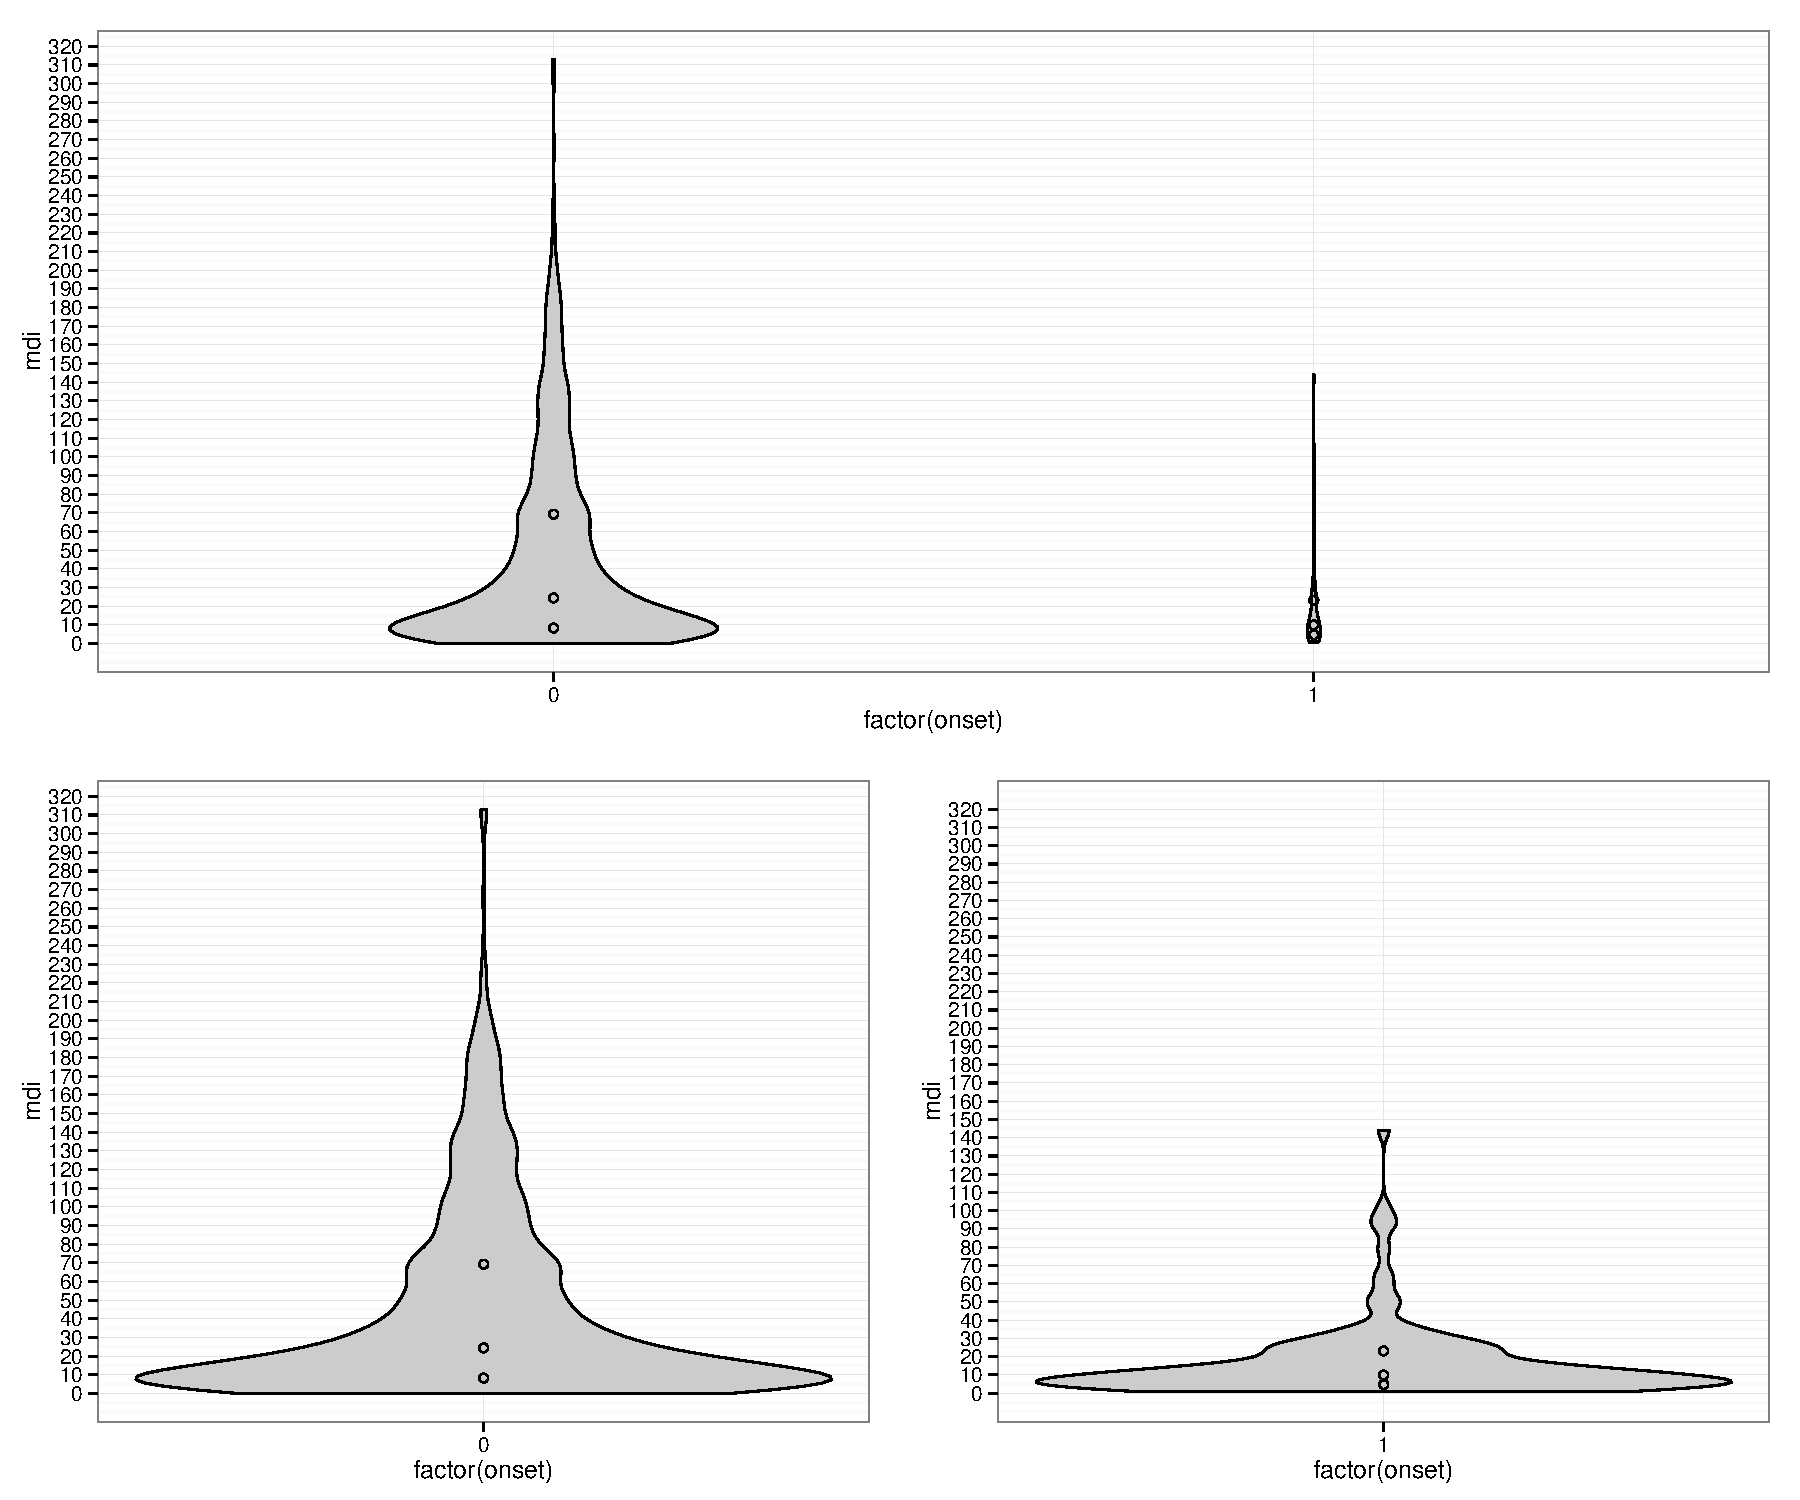
\includegraphics{media_civil_war_files/figure-markdown/violinplot.pdf}
\caption{Violin plot of media density for all civil war onsets}
\end{figure}

These plots illustrate three important facts about the distributions of
civil war onset and mass media density in this sample of countries
between 1945-1999. First, these distributions challenge a key rationale
for questioning the qualitative evidence that mass media plays a causal
role in generating civil war onsets. Warren argues that those cases in
which mass media are known to have played a significant role in civil
war--cases such as Yugoslavia and Rwanda in the early 1990s (MDIs of
40.5 and 6.3, respectively) are unrepresentatively low levels of mass
media density (Warren 2014, 132). Warren argues that because analysts
have effectively selected these cases on the dependent variable, they
``observe mass communication behavior only in those countries that are
experiencing the outbreak of large-scale civil conflict'' (Warren 2014,
132). The implication is that the positive association between mass
media and civil war established by previous qualitative research is
spurious and that ``expanding our focus to the full universe of cases
reveals quite a different picture'' (Warren 2014, 123).

Illustrating the entire distribution of the full universe of cases,
however, Figure 2 illustrates that cases such as Yugoslavia and Rwanda
are indeed fairly typical country-years in the period 1945-1999. While
it is true that in these cases mass media density is below the global
average \emph{in that year}, these cases bracket the global median of
MDI (23.924) by less than half of one standard deviation (25.9347) on
either side. Thus, some of the well-known cases which illustrate the
bellicose effects of mass media are indeed highly representative of MDI
levels globally in the post-war period until 1999.

Second, if there is a problem of unrepresentativeness it is that the
extreme right-skew of MDI in peaceful country-years may drive a
disproportionate amount of the negative association between levels of
MDI and civil war. Figure 2 illustrates that no civil war has ever been
observed in any country-year characterized by MDI greater than roughly
150, but these are highly unrepresentative cases (in the 94\%
percentile). This is important because it indicates that estimates of
the relationship between mass media and civil war may be driven by a
minority of cases with uncommonly high values on the independent
variable, leading to misleading inferences.

Finally, civil wars are most frequently observed at low but positive
levels of MDI compared to the zero level. This is contrary to what we
would expect from the general pacification theory; if the relationship
between MDI and civil war onset is negative and monotonic, we would
expect civil wars to be more frequent at the zero level of mass media
density. Rather, the distribution suggests the possibility of
non-linearity at low levels of mass media density, precisely as
predicted by the war-before-peace theory.

\subsection{Considering Non-Linearity with Semi-Parametric
Regression}\label{considering-non-linearity-with-semi-parametric-regression}

To test whether mass media density has a non-linear effect on civil war
onset, this section compares the fit of a baseline logistic regression
replicated from Warren (not displayed) with an additive semi-parametric
regression model identical in every respect except that the effect of
MDI is estimated with a nonparametric smooth allowing it to vary at
different levels of MDI. Specifically, I estimate the model

\[ Onset_{it} = \alpha + f_1 (LogMDI_{it}) + Controls_{it} \beta  + \varepsilon_{it} \]

where the partial-regression function $f_1 (\cdot)$ is fit by a
smoothing spline (Fox 2002; Wood 2000) and $CONTROLS_{it}$ is the vector
of control variables used in Warren's original models. The number of
smoothing splines is determined by generalized cross validation as part
of the estimation procedure.\footnote{The model was estimated using the
  function \emph{gam} in the \emph{mgcv} package for R.}

Figure 3 plots the value of the smooth terms for each level of the
logarithm of MDI, i.e.~the estimated effect of the logarithm of MDI on
the probability of civil war onset across its range. The result is
consistent with Hypothesis 1: MDI is positively associated with civil
war onset up to a threshold, the estimated effect slightly increasing up
to that threshold, before changing direction and decreasing. To
determine whether the non-linear fit is superior to the linear fit, a
simple analysis of variance (ANOVA) can be used to contrast the deviance
of each model. Table 1 displays the results, which suggest that the
non-linear fit reduces the deviance by 18 and is statistically
significant.

\begin{figure}[htbp]
\centering
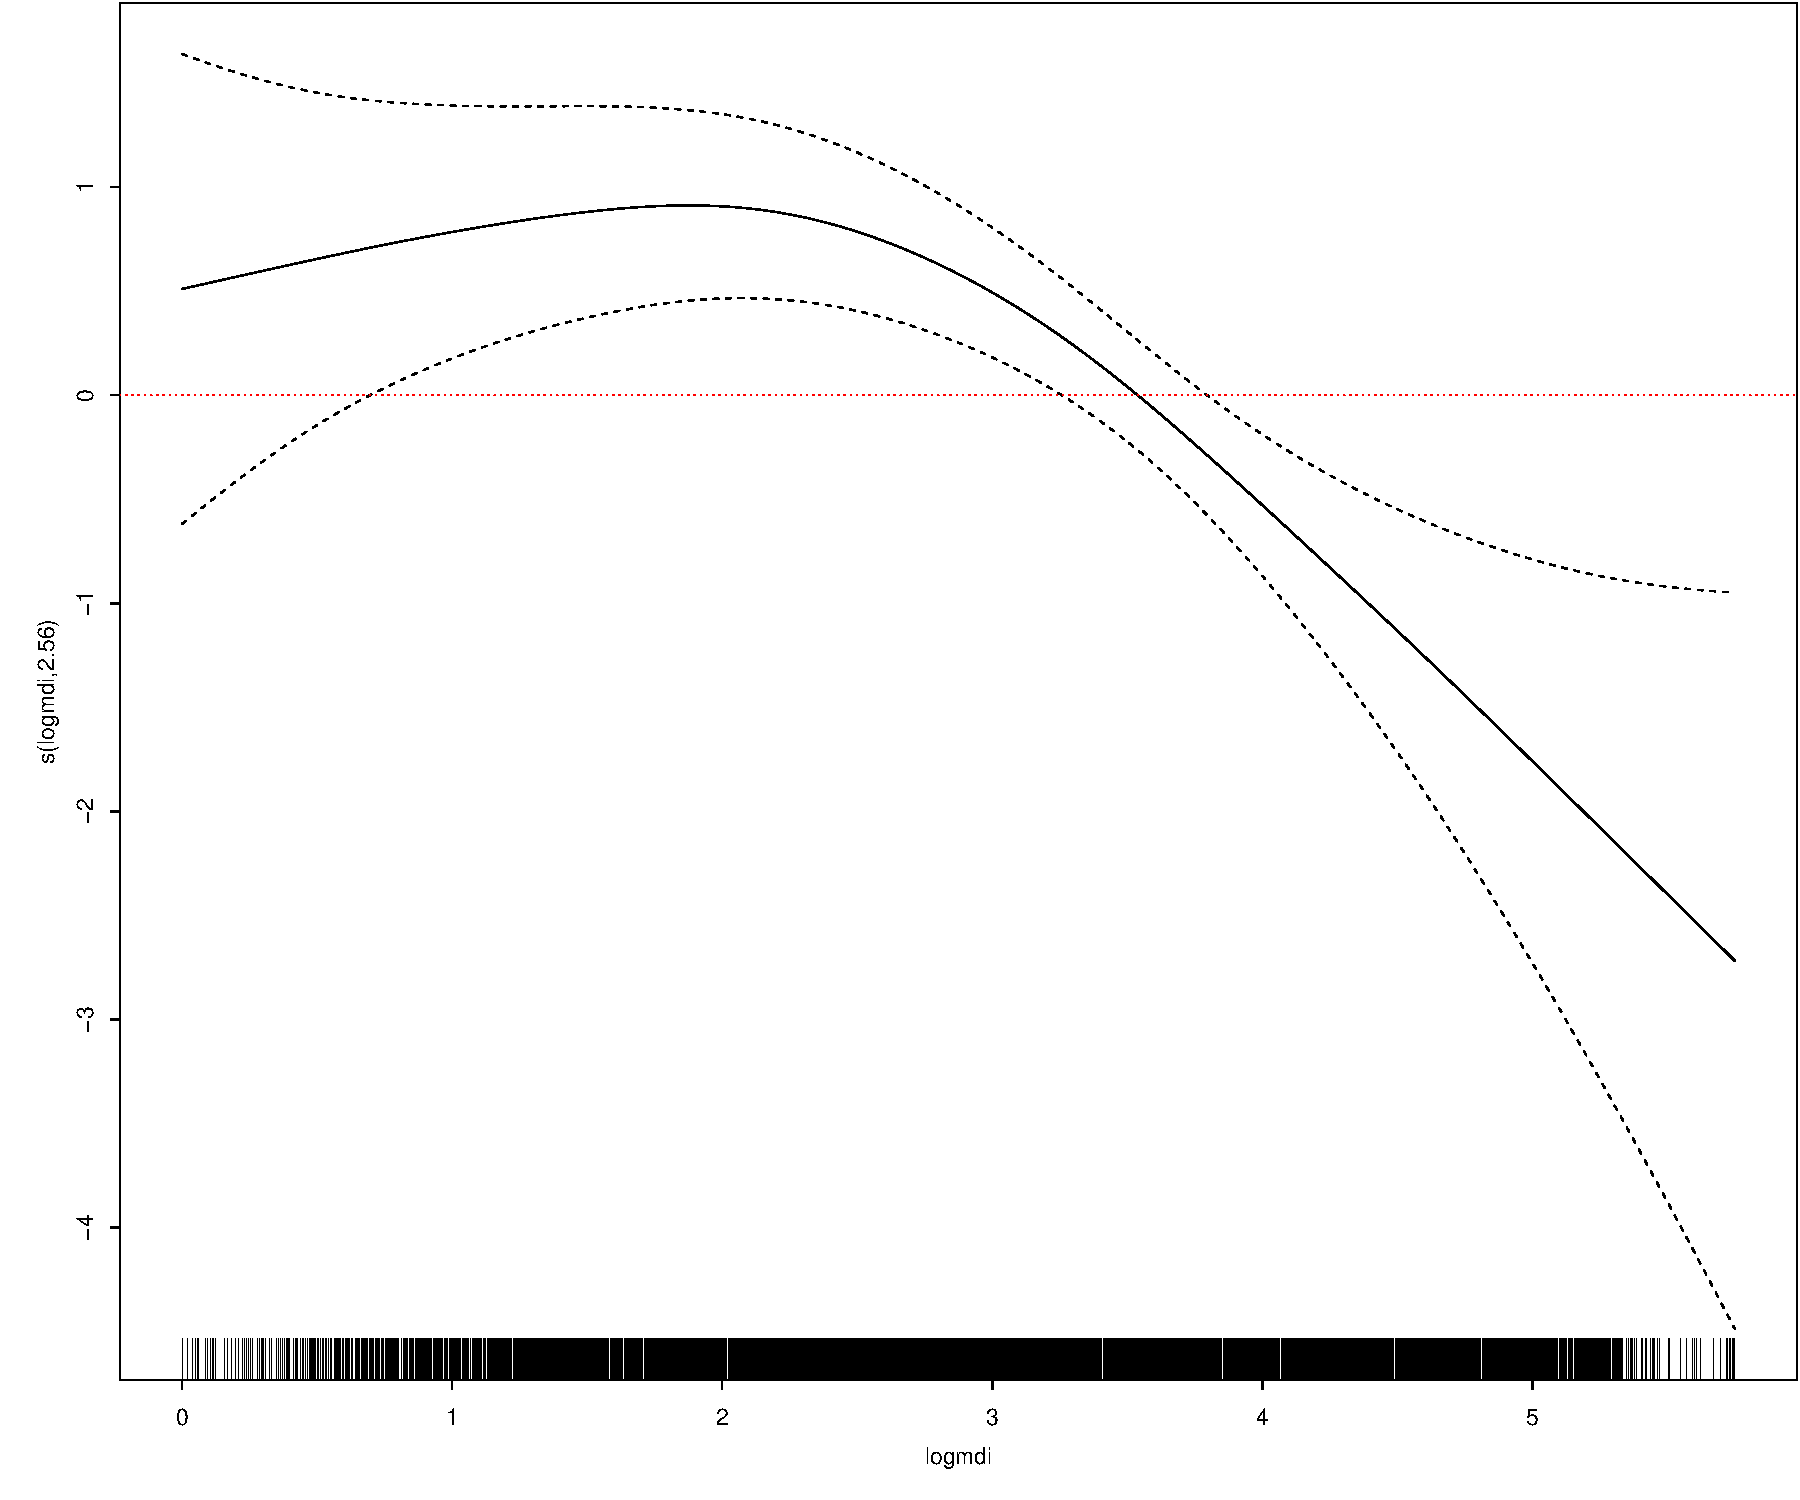
\includegraphics{media_civil_war_files/figure-markdown/nonlinear-plot.pdf}
\caption{The Non-Linear Effect of MDI on Civil War Across Levels of MDI}
\end{figure}

\begin{table}[!htbp] \centering 
  \caption{ANOVA Comparing Linear and Non-Linear Effects of MDI on Civil War Onset} 
  \label{} 
\footnotesize 
\begin{tabular}{@{\extracolsep{5pt}} cccccc} 
\\[-1.8ex]\hline \\[-1.8ex] 
 & RESID. DF & RESID. DEV & DF & DEVIANCE & P-VALUE \\ 
\hline \\[-1.8ex] 
1 & $5,884$ & $1,070.00$ & $$ & $$ & $$ \\ 
2 & $5,882.00$ & $1,052.00$ & $1.56$ & $17.90$ & $0.0001$ \\ 
\hline \\[-1.8ex] 
\end{tabular} 
\end{table}

\subsection{Estimating the Effect of Mass Media Density Before and After
the Threshold of Mass
Communications}\label{estimating-the-effect-of-mass-media-density-before-and-after-the-threshold-of-mass-communications}

To further test the hypothesis that MDI increases the likelihood of
civil war before it is sufficiently high to represent a mass
communications system (and to obtain a parsimonious estimate of the
effect size), I estimate a series of traditional parametric regressions.
I begin by creating a subset of the original sample containing only
country-years with MDI levels below the inflection point identified by
the non-linear regression (when logged MDI is equal to about 2, or an
MDI level of about 6.3885). While it is reasonable to think such a low
threshold might only correspond to a substantively trivial number of
cases, on the contrary, this subset contains 1360 cases or about 20\% of
the original sample. I estimate traditional logistic regressions all of
which are variations on the form

\[ Onset_{it} = \alpha + MDI_{it} \beta_1 + Controls_{it} \beta_2  + \varepsilon_{it} \]

and where all the variables are the same as in the previous equation,
with the exception that \emph{MDI} is not logged.

Table 2 displays the results with adjustment for rare events (Gary King
and Zeng 2001).\footnote{Traditional logistic regression estimated by
  maximum-likelihood would likely underestimate the probability of civil
  war onsets because civil wars begin in relatively very few
  country-years. There are 119 (2.0588\%) onsets in the full sample and
  41 (3.2437\%) in the subset of low-MDI country-years.} Before
analysis, I subtracted the mean from each continuous independent
variable and then divided it by two standard deviations so that all
resulting coefficients are readily comparable.\footnote{For continuous
  independent variables, the coefficient indicates the change in
  log-odds of a civil war beginning due to a two standard deviation
  increase from the mean of the independent variable; for dichotomous
  variables, the coefficient reflects the change in log-odds of a civil
  war beginning due to a change from 0 to 1 on the dichotomous variable,
  which is roughly equivalent to a two-standard deviation change in a
  continuous variable (Gelman 2008).}

The first two columns of the following table display the results of a
baseline model which replicates Warren's original findings (Model 1) and
the same model estimated on the subset of country-years below the median
level of MDI (23.924). While Model 1 successfully replicates Warren's
main finding with a negative and statistically significant coefficient
for MDI levels, Model 2 indicates that this coefficient is not
statistically significant for country-years below the median level of
MDI. The third column estimates a model nearly equivalent to the first
two but only for country-years below the 20th percentile of MDI, roughly
the inflection point suggested by the semi-parametric regression
estimated in the previous stage of analysis (the logarithm of MDI equal
to 2).\footnote{I use the 20th percentile of MDI because it is a
  convenient and conventional cutoff for segmenting distributions; it is
  slightly less than a logarithm of 2.} Distinct from Models 1 and 2,
the independent variable of interest in Model 3 is the variable
capturing year-to-year changes in MDI rather than levels of MDI. Levels
of MDI are not included as an independent variable because Model 3 is
effectively already controlling for the level of MDI by restricting
attention to the 20th percentile of media density. The coefficient for
$\Delta$$MDI_{t-1}$ is negative and statistically significant, as
predicted by Hypothesis 1.

The results suggest that the general pacification theory would
significantly underestimate the probability of civil war onset in
countries first observing the introduction and early spread of mass
media. Warren's baseline model (Model 1) would lead us to predict that a
country moving from zero MDI to the 20th percentile (5.4992) would, on
average, cause the probability of civil war onset to decrease by
-0.0047, from an already quite low 0.0355. However, when we estimate the
same model on only those country-years in the 20th percentile of mass
media density (Model 3), simulations suggest an increase of 5.4992 would
cause the probability of civil war onset to increase by an average of
0.6309, from 0.0208 to 0.6517.\footnote{All simulations and predicted
  probability plots were generated using the R package \emph{Zelig}
  (Imai, King, and Lau 2009).}

\begin{table}[!htbp] \centering 
  \caption{Early Growth of Media Density Compared to Media Density in General} 
  \label{} 
\scriptsize 
\begin{tabular}{@{\extracolsep{5pt}}lccc} 
\\[-1.8ex]\hline \\[-1.8ex] 
 & Warren & <= Median MDI & <= 20th Percentile MDI \\ 
\\[-1.8ex] & (1) & (2) & (3)\\ 
\hline \\[-1.8ex] 
 MDI$_{t-1}$ & $-$2.64$^{***}$ & $-$3.27 &  \\ 
  & (0.71) & (2.38) &  \\ 
  $\Delta$MDI$_{t-1}$ &  &  & 0.67$^{**}$ \\ 
  &  &  & (0.31) \\ 
  GDP PER CAPITA$_{t-1}$ & $-$0.09 & $-$0.33 & $-$1.04$^{**}$ \\ 
  & (0.36) & (0.48) & (0.45) \\ 
  AREA$_{t-1}$ & $-$0.31 & $-$0.19 & 0.13 \\ 
  & (0.32) & (0.39) & (0.57) \\ 
  MOUNTAINOUS$_{t-1}$ & 0.45$^{*}$ & 0.41 & $-$0.07 \\ 
  & (0.24) & (0.27) & (0.40) \\ 
  POPULATION$_{t-1}$ & 0.80$^{***}$ & 0.75$^{***}$ & 0.78$^{*}$ \\ 
  & (0.25) & (0.29) & (0.46) \\ 
  OIL EXPORTER$_{t-1}$ & 0.76$^{***}$ & 0.73$^{**}$ & 1.74$^{***}$ \\ 
  & (0.28) & (0.36) & (0.57) \\ 
  DEMOCRACY$_{t-1}$ & 2.68$^{**}$ & 2.68$^{*}$ & 1.93 \\ 
  & (1.15) & (1.38) & (1.61) \\ 
  DEMOCRACY$^2$$_{t-1}$ & $-$2.54$^{**}$ & $-$2.19 & $-$1.39 \\ 
  & (1.22) & (1.49) & (1.55) \\ 
  ETHNIC FRAC.$_{t-1}$ & 0.11 & $-$0.09 & $-$0.40 \\ 
  & (0.21) & (0.24) & (0.41) \\ 
  RELIGIOUS FRAC.$_{t-1}$ & 0.60$^{***}$ & 0.56$^{**}$ & 0.47 \\ 
  & (0.23) & (0.27) & (0.39) \\ 
  PEACE YEARS$_{t-1}$ & $-$1.89 & $-$2.85 & $-$0.20 \\ 
  & (2.57) & (2.94) & (2.92) \\ 
  SPLINE 1 & $-$0.55 & $-$7.95 & 3.46 \\ 
  & (15.70) & (18.14) & (14.83) \\ 
  SPLINE 2 & $-$5.22 & 3.52 & $-$5.29 \\ 
  & (18.23) & (21.66) & (16.95) \\ 
  SPLINE 3 & 3.49 & 0.90 & 1.20 \\ 
  & (5.57) & (7.30) & (5.28) \\ 
  CONSTANT & $-$4.54$^{***}$ & $-$4.66$^{***}$ & $-$3.86$^{***}$ \\ 
  & (0.18) & (0.78) & (0.25) \\ 
 \textit{Observations} & 5,899 & 2,950 & 1,220 \\ 
\textit{Log likelihood} & $-$527.50 & $-$373.10 & $-$148.00 \\ 
\textit{Akaike information criterion} & 1,085.00 & 776.10 & 326.10 \\ 
\hline \\[-1.8ex] 
\textit{Notes:} & \multicolumn{3}{l}{$^{***}$p $<$ .01; $^{**}$p $<$ .05; $^{*}$p $<$ .1} \\ 
\end{tabular} 
\end{table}

While the difference between zero MDI and the 20th percentile of 5.4992
is a useful yardstick with respect to the entire range of \emph{levels}
observed in the sample, the mean year-to-year change observed in the
subset of pre-mass communications systems is only 0.2118 and the maximum
is only 2.77. Thus, to gain a more realistic sense of how the early
spread of mass media shapes civil war onset, and to better compare the
substantive implications of the general pacification effect with the
war-before-peace effect, Figures 4 and 5 display the predicted
probability of civil war onset given different values of MDI levels and
year-to-year MDI changes, respectively, across their historically
observed ranges.

Considering all communications systems, the predicted probability of
civil war onset decreases from about .03 at the zero level of MDI to
roughly zero for any level of MDI greater than about 150, on average.
However, considering only pre-mass communications systems, a 1-point
change in MDI would cause the probability of civil war onset to increase
by an average of 0.0311, from 0.021 to 0.052. A 2.5-point change in MDI
would cause the probability of civil war onset to increase by an average
of 0.1955, from 0.0206 to 0.2161. Figures 4 and 5 also highlight the
essential assymetry of estimating negative versus positive effects on a
rare event. The pacifying effect of levels of MDI as identified by
Warren is an inherently small effect because the probability of
observing civil war onset is already very small in general. However, the
size of the war-before-peace effect is notably larger and represents a
more substantively salient risk for this same reason.

\clearpage

\begin{figure} 
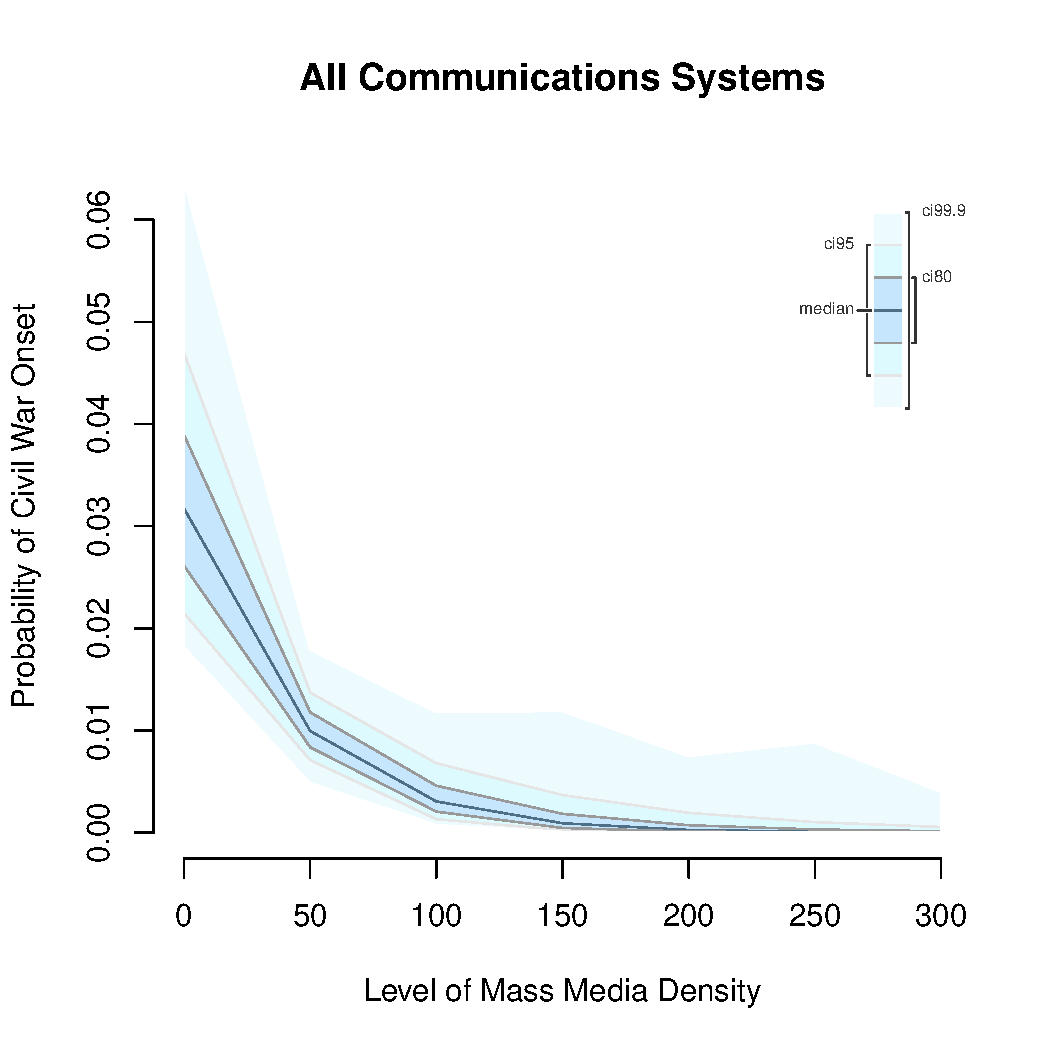
\includegraphics{figure/mdi_effect.pdf} 
\caption{Predicted probability of civil war onset given levels of media density} 
\label{myFigur} 
\end{figure}

\clearpage

\begin{figure} 
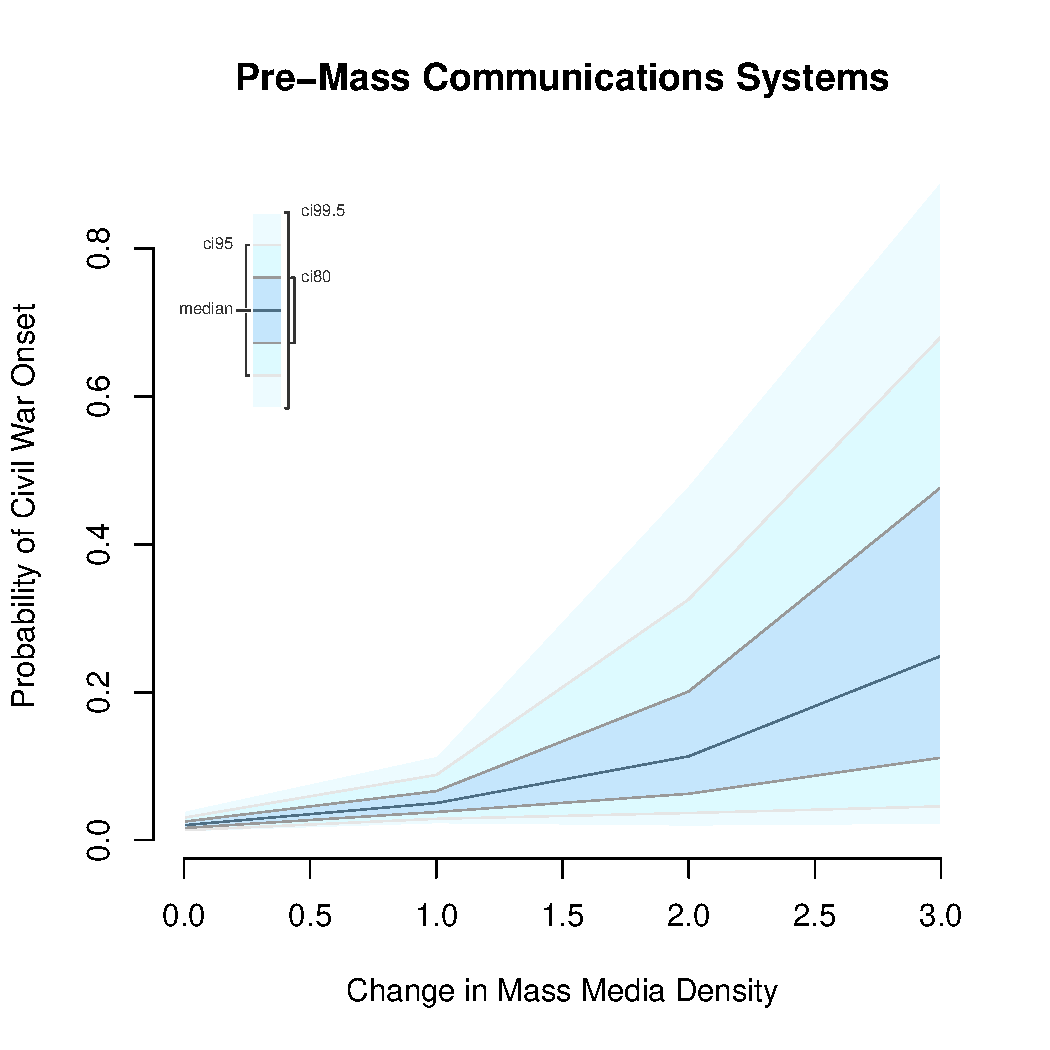
\includegraphics{figure/d_mdi_effect.pdf} 
\caption{Predicted probability of civil war onset given changes in media density} 
\label{myFigz} 
\end{figure}

\subsection{Mass Media Density and Civil Wars at the International
Level}\label{mass-media-density-and-civil-wars-at-the-international-level}

Table 3 models the number of civil war onsets in the international
system each year using the negative binomial distribution, the
appropriate distribution for modelling event counts. Formally, the
equation is

\[ Onsets_{i} = \alpha + TV_{i} \beta_1 + \Delta TV_{i} \beta_2 + Controls_{i} \beta_3  + \varepsilon_{i}, \]

where the dependent variable \emph{Onsets} is the number of civil wars
which begin in year \emph{i}, and the independent variables of interest
are the levels and first differences of television density (\emph{TV}
and $\Delta TV$, respectively).

Model 1 is a baseline model. Model 2 includes controls variables
\emph{WW1}, \emph{WW2}, and \emph{COLD WAR.} Model 3 adds to these the
control variable \emph{IMPUTED.} Each model provides evidence for
Hypothesis 2, that with respect to the international system in
historical perspective, year-to-year increases in television density are
positively associated with the number of civil war onsets in the
following year. Figure 6 illustrates the expected change in global civil
war onsets for a range of changes in the global mean of television
density. These results are consistent with the evidence presented above,
reflecting that year-to-year increases in media density within low
levels increase the likelihood of civil war, even if media density has a
pacifying effect in the long-run. Interestingly, the international-level
models do not provide much evidence for a long-term pacifying effect
from levels of television density, as the negative effect is no longer
statistically significant after controlling for \emph{WW1}, \emph{WW2},
and \emph{COLD WAR}. However, this could be for the reason that global
television density remains relatively low and has not yet reached the
threshold at which its pacifying effects would become observable at the
level of the international system.

\begin{figure}[htbp]
\centering
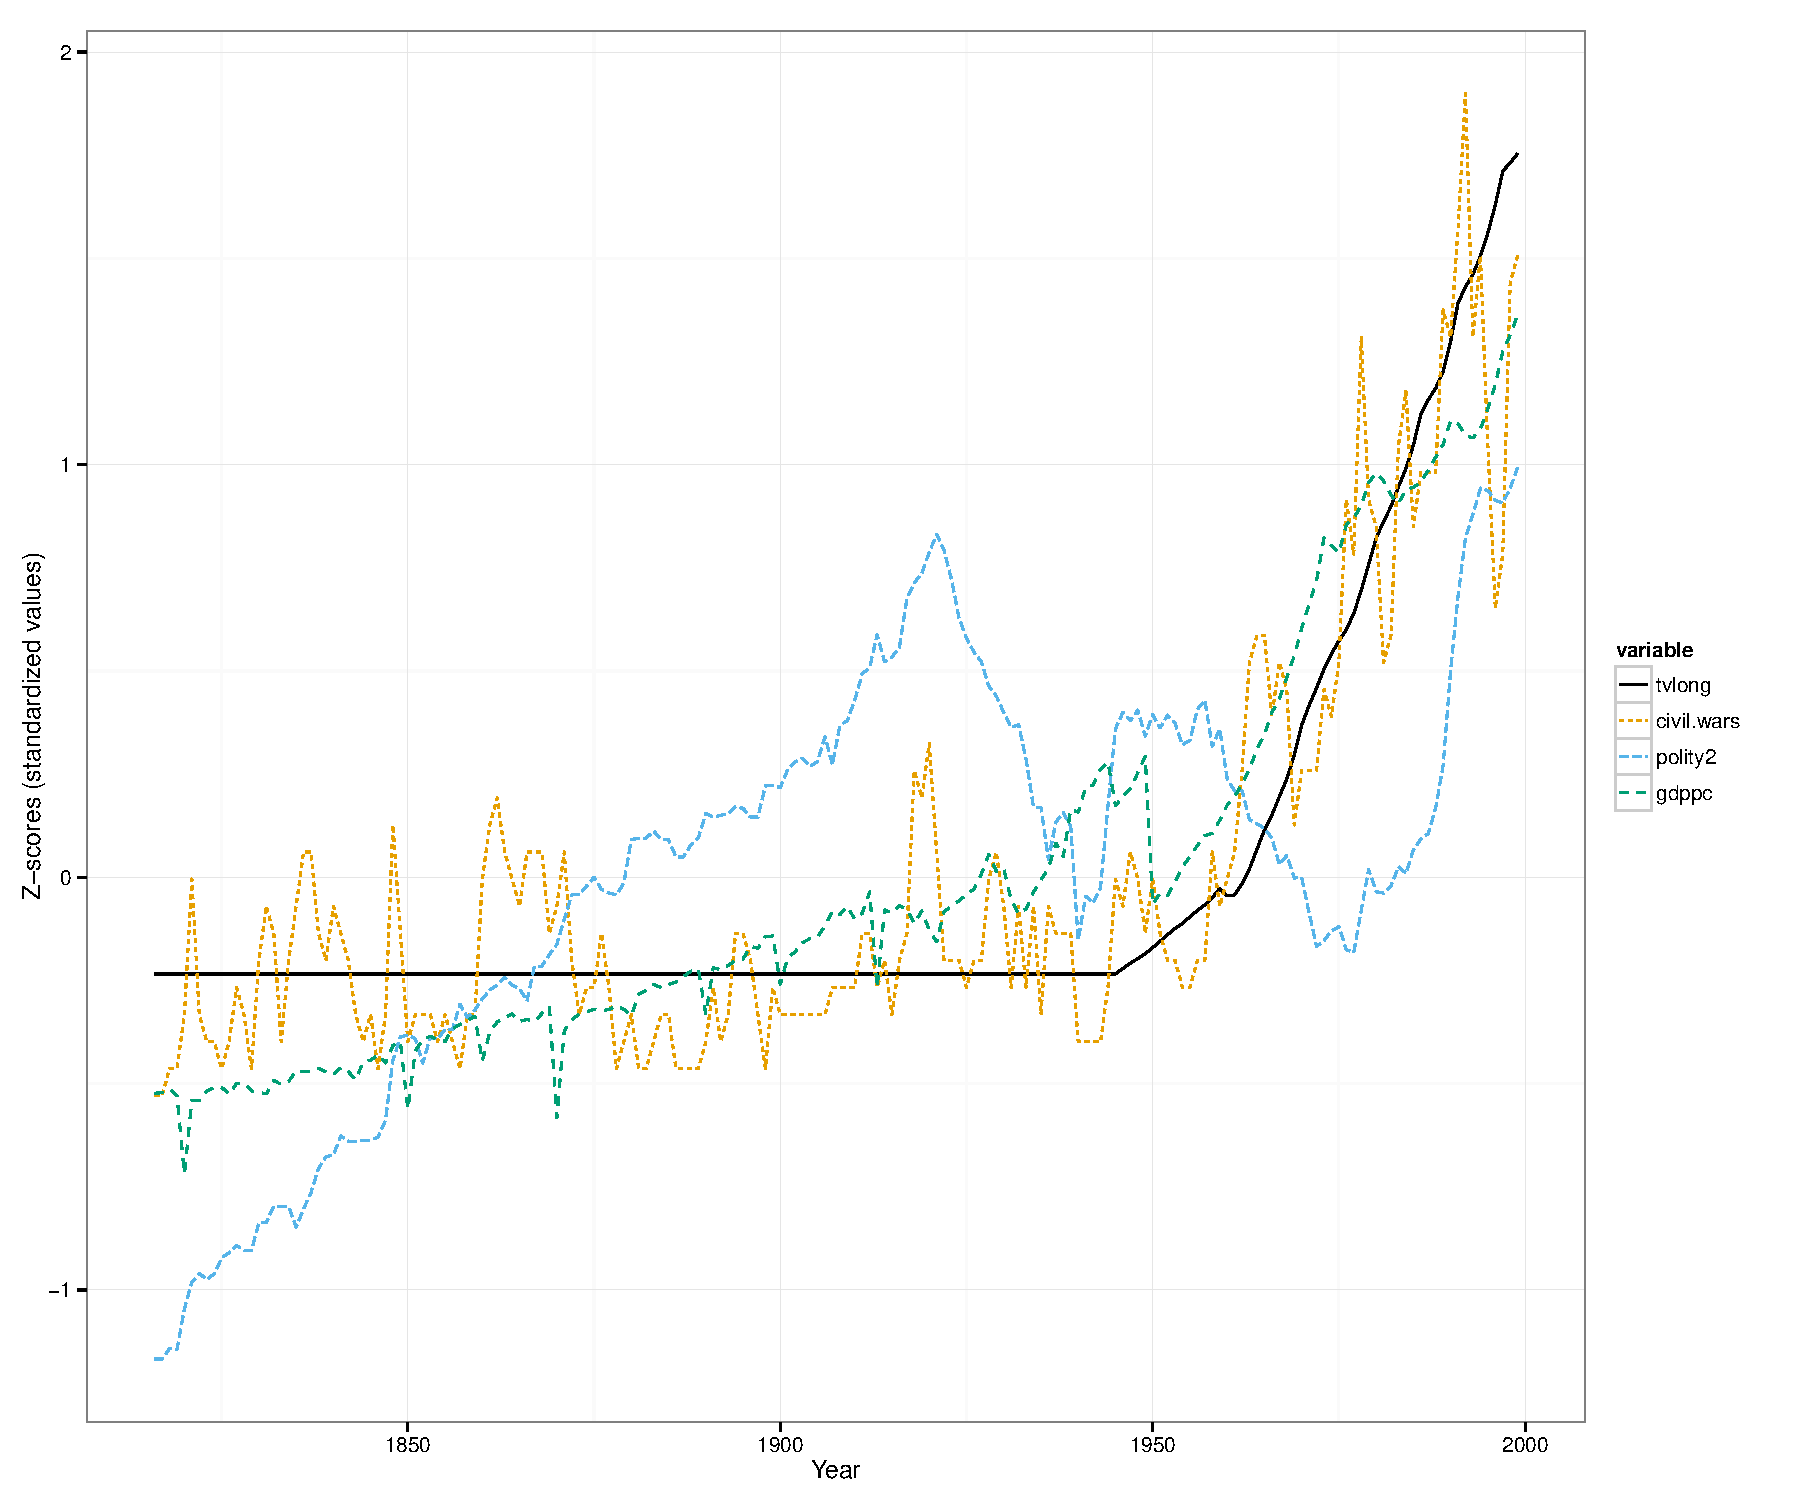
\includegraphics{media_civil_war_files/figure-markdown/longrunplot.pdf}
\caption{TV, Democracy, Economic Growth, and Civil Wars Globally,
1816-1999}
\end{figure}

Simulations suggest that a .5 increase in the global mean TV density (an
increase equal to two standard deviations above the mean yearly
increase) would generate approximately one extra civil war per year on
average (0.9689, from 1.5175 to 2.4864).

\begin{table}[!htbp] \centering 
  \caption{International-Level Regressions} 
  \label{} 
\scriptsize 
\begin{tabular}{@{\extracolsep{5pt}}lccc} 
\\[-1.8ex]\hline \\[-1.8ex] 
\\[-1.8ex] & \multicolumn{3}{c}{onsets} \\ 
\\[-1.8ex] & (1) & (2) & (3)\\ 
\hline \\[-1.8ex] 
 TV$_{t-1}$ & $-$0.91$^{**}$ & $-$0.66 & $-$0.60 \\ 
  & (0.37) & (0.40) & (0.40) \\ 
  $\Delta$TV & 0.33$^{**}$ & 0.42$^{***}$ & 0.46$^{***}$ \\ 
  & (0.15) & (0.16) & (0.16) \\ 
  GDP PER CAPITA$_{t-1}$ & $-$0.07 & $-$0.03 & $-$0.24 \\ 
  & (0.51) & (0.57) & (0.57) \\ 
  $\Delta$GDP PER CAPITA & $-$0.01 & $-$0.03 & $-$0.06 \\ 
  & (0.06) & (0.06) & (0.06) \\ 
  DEMOCRACY$_{t-1}$ & 0.25 & 0.94$^{***}$ & 0.99$^{***}$ \\ 
  & (0.19) & (0.27) & (0.27) \\ 
  $\Delta$DEMOCRACY & $-$0.19$^{*}$ & $-$0.18$^{*}$ & $-$0.21$^{**}$ \\ 
  & (0.10) & (0.11) & (0.11) \\ 
  DEMOCRACY$^2_{t-1}$ & 0.20 & 0.36$^{*}$ & 0.41$^{**}$ \\ 
  & (0.16) & (0.20) & (0.19) \\ 
  CIVIL WARS & 0.91$^{***}$ & 0.93$^{***}$ & 0.95$^{***}$ \\ 
  & (0.24) & (0.25) & (0.25) \\ 
  ONSETS$_{t-1}$ & 0.90$^{***}$ & 0.95$^{***}$ & 0.97$^{***}$ \\ 
  & (0.16) & (0.16) & (0.16) \\ 
  $\Delta$ONSETS & 0.16$^{***}$ & 0.17$^{***}$ & 0.17$^{***}$ \\ 
  & (0.02) & (0.02) & (0.02) \\ 
  STATES & 0.24 & 0.37 & 0.49 \\ 
  & (0.57) & (0.59) & (0.59) \\ 
  YEAR & $-$0.28 & $-$1.14$^{*}$ & $-$1.05 \\ 
  & (0.56) & (0.69) & (0.69) \\ 
  WWI &  & $-$0.12 & $-$0.17 \\ 
  &  & (0.18) & (0.17) \\ 
  WWII &  & 0.41$^{*}$ & 1.57$^{***}$ \\ 
  &  & (0.22) & (0.34) \\ 
  COLD WAR &  & $-$0.92$^{***}$ & $-$1.01$^{***}$ \\ 
  &  & (0.22) & (0.22) \\ 
  IMPUTED &  &  & 1.23$^{***}$ \\ 
  &  &  & (0.36) \\ 
  CONSTANT & 0.53$^{***}$ & 0.57$^{***}$ & $-$0.28 \\ 
  & (0.04) & (0.08) & (0.26) \\ 
 \textit{Observations} & 182 & 182 & 182 \\ 
\textit{Log likelihood} & $-$260.00 & $-$257.00 & $-$256.10 \\ 
$\theta$ & 45,133.00  (484,186.00) & 44,773.00  (456,964.00) & 45,671.00  (465,362.00) \\ 
\textit{Akaike information criterion} & 545.90 & 546.00 & 546.20 \\ 
\hline \\[-1.8ex] 
\textit{Notes:} & \multicolumn{3}{l}{$^{***}$p $<$ .01; $^{**}$p $<$ .05; $^{*}$p $<$ .1} \\ 
\end{tabular} 
\end{table}

\clearpage

\begin{figure} 
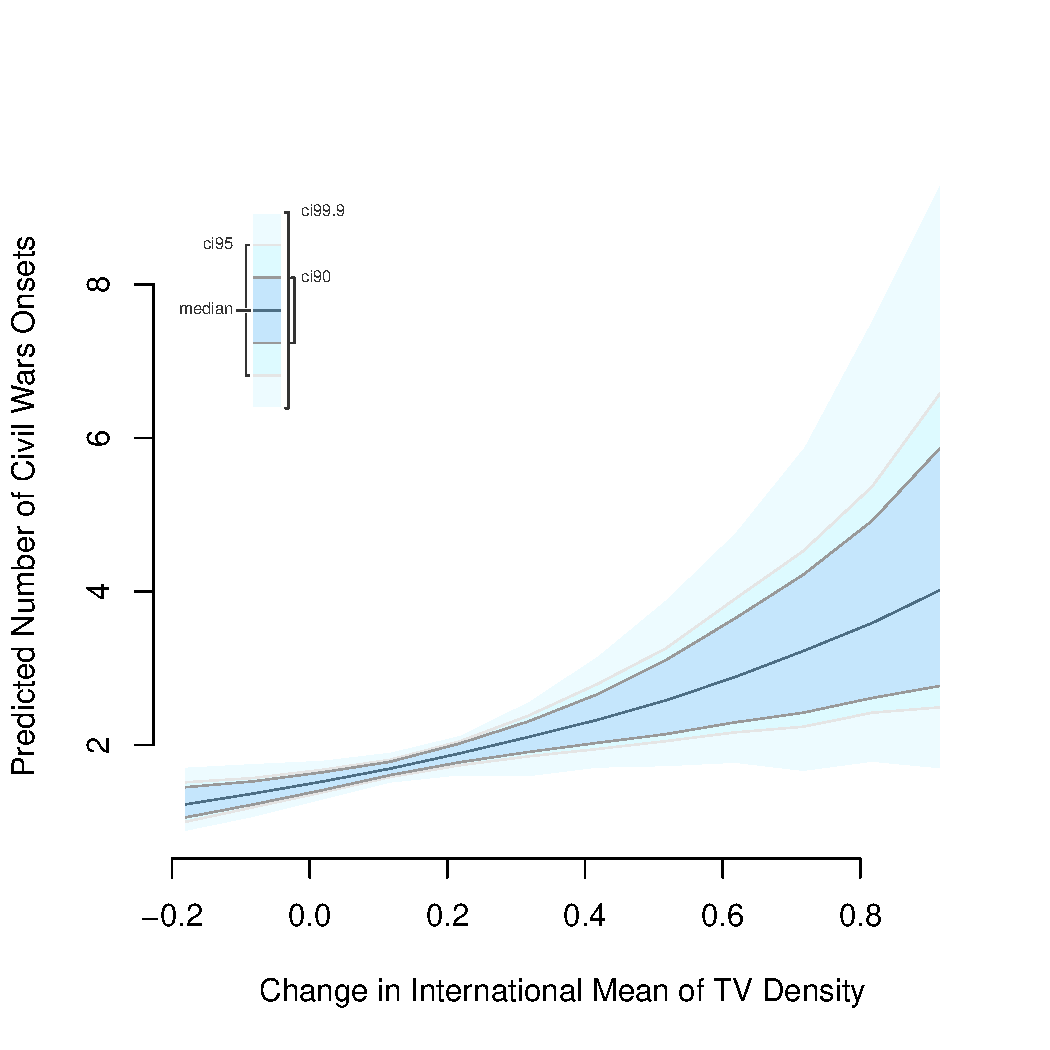
\includegraphics{figure/dtv_effect.pdf} 
\caption{Predicted number of civil war onsets given changes in global TV density} 
\label{myFigur} 
\end{figure}

\section{Conclusion}\label{conclusion}

This research note synthesizes conflicting evidence on the relationship
between mass media and civil war onset by hypothesizing a non-linear
relationship. After mass media density crosses the threshold
constituting a mass communications system, communicative economies of
scale are such that every further increase in mass media density
increases the communicative powers of the state, further deterring
insurgents, and thus further decreasing the likelihood of civil war
onset. However, when mass media density is below the threshold
constituting a mass communications system, increases in mass media
density significantly increase the likelihood of civil war onset as the
approach of a mass communications system represents a ``now or never''
situation for potential insurgents. The argument is supported by
semi-parametric and traditional parametric regression analyses on a
large panel of countries between 1945 and 1999 and international-level
time-series beginning in 1816.

The implications are critical for political scientists as well as
policymakers, activists, and other political actors concerned with
issues of media, communications, and civil violence. First, the
implications are substantively critical for scholars, policymakers and
other political practitioners interested in the causes of civil war
because the most recent previous evidence would lead observers to
underestimate the risk of civil war within countries experiencing the
early spread of mass media. By demonstrating the bellicose effects of
mass media in precisely such situations, this research note draws
attention to a unique source of civil war risk which has been poorly
understood by previous research. Second, this research note highlights
that in the politics of mass communications, considerations of
non-linearity are likely to be especially important. Assuming linear
relationships between independent and dependent variables is not always
warranted and can lead to substantively different predictions than those
generated by models which account for non-linearity. The findings
presented here will be of interest in particular to those scholars in
the burgeoning field of ICT and political conflict research who are
building an increasingly ``rich theory'' of context-conditional findings
(Lyall and Dafoe 2015). This research note contributes to this current
of research both theoretically and empirically, by highlighting the
theoretical importance of non-linearities in these types of phenomena
and by providing an improved empirical accounting of mass media in
patterns of civil war onset.

\clearpage

\section{Supplementary Information}\label{supplementary-information}

\subsection{Contents}\label{contents}

\begin{enumerate}
\def\labelenumi{\arabic{enumi}.}
\itemsep1pt\parskip0pt\parsep0pt
\item
  Summary visualization
\item
  Tests of stationarity
\item
  Semi-parametric regressions on disaggregated media density
\end{enumerate}

\begin{figure}[htbp]
\centering
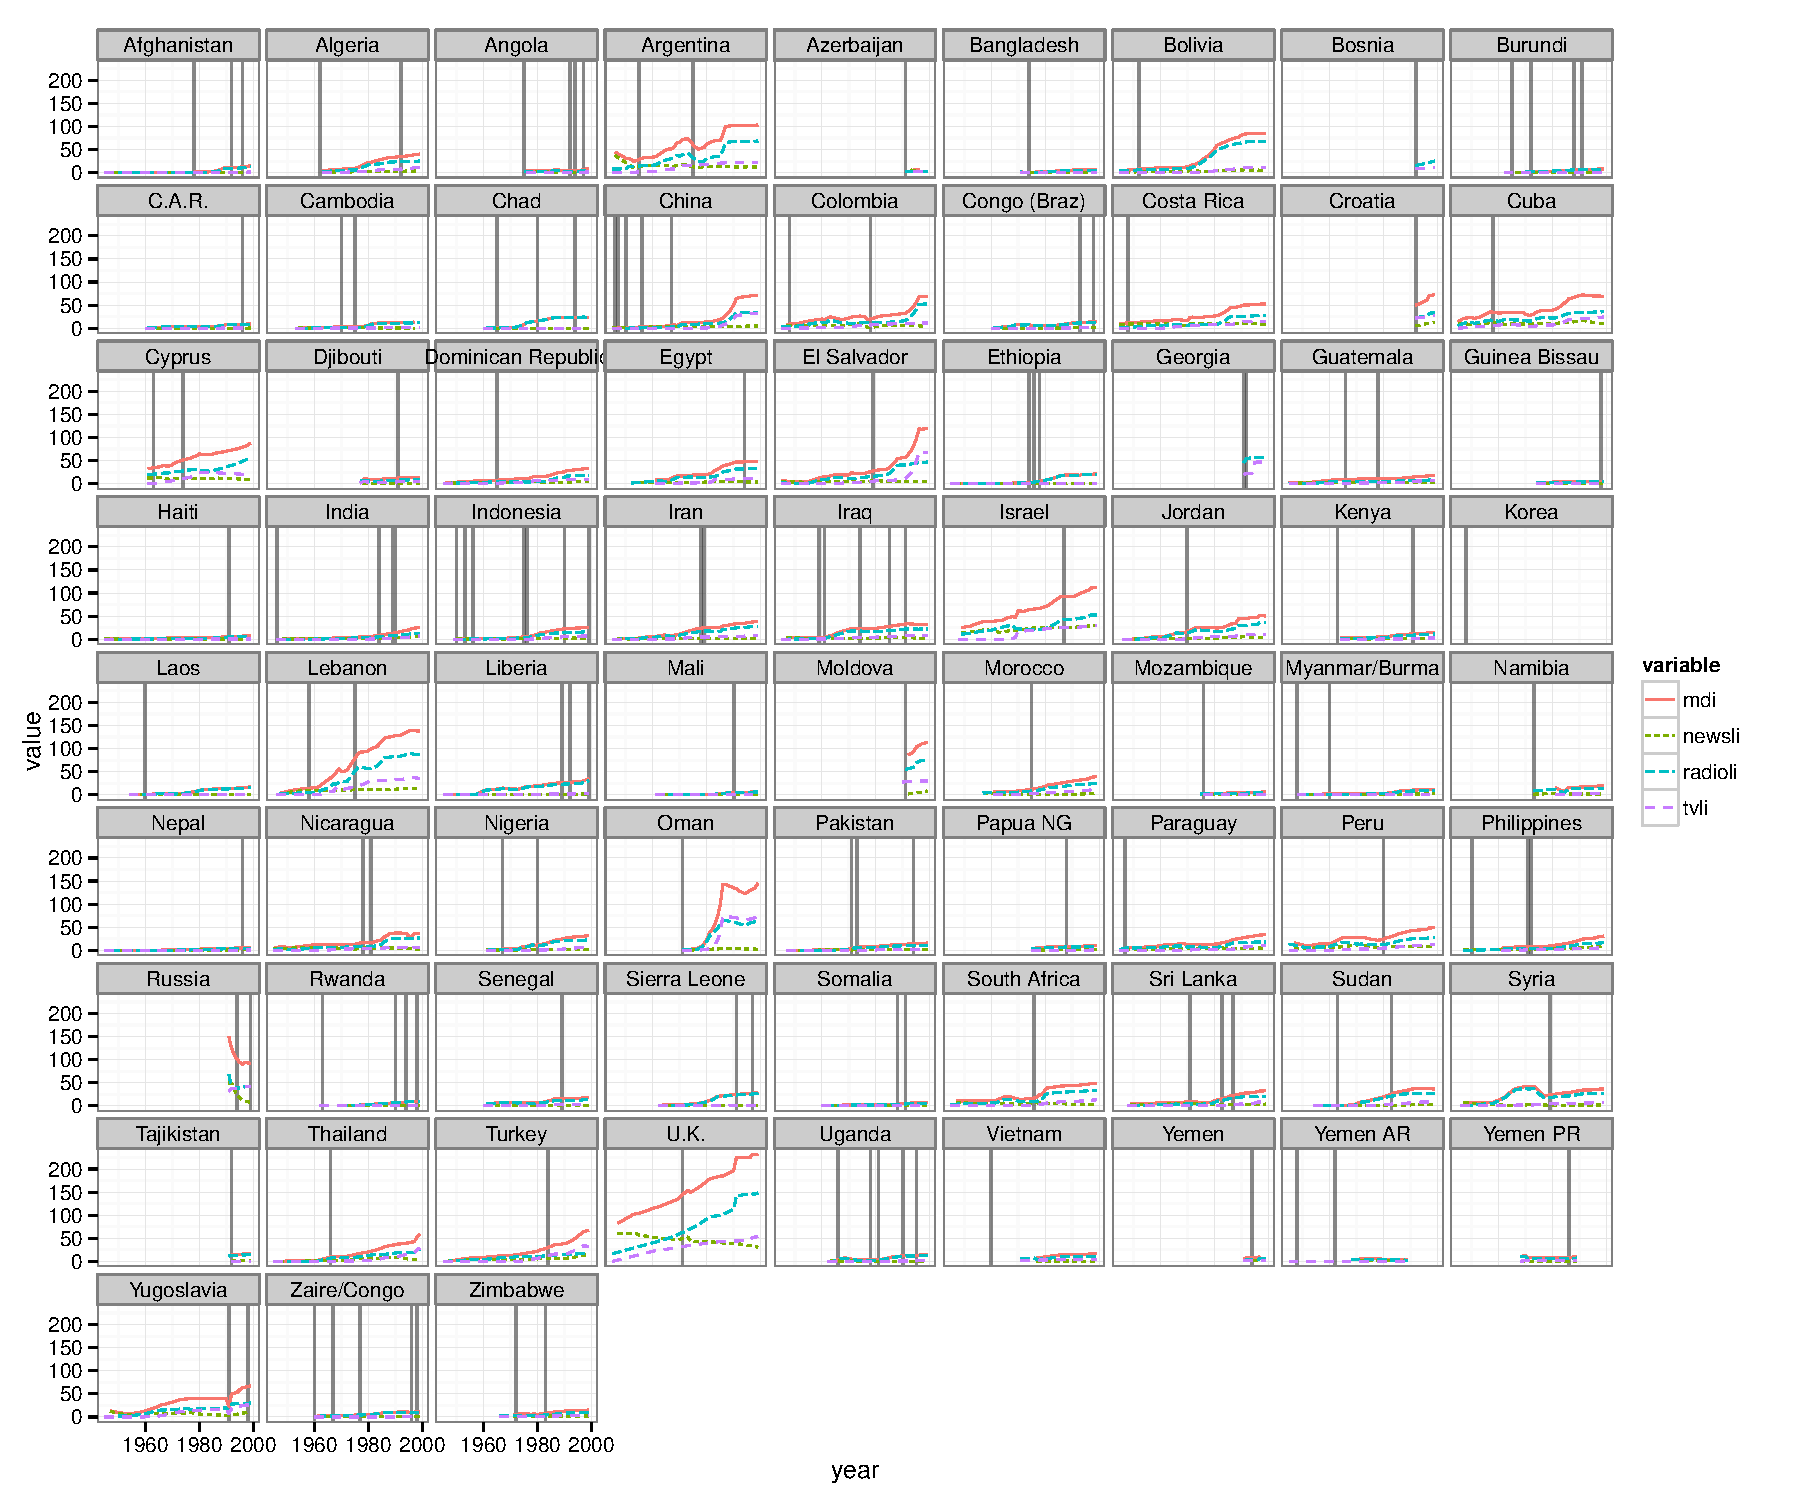
\includegraphics{media_civil_war_files/figure-markdown/full_panel_plot.pdf}
\caption{Disaggregated media density and all civil war onsets over time,
by country}
\end{figure}

\subsubsection{Tests of Stationarity}\label{tests-of-stationarity}

The Levin-Lin-Chu statistic is a standard test for the presence of a
unit root, otherwise known as non-stationarity or integration of order
I(1), in a time series variable observed across multiple cross-sectional
units. The Im-Pesaran-Shin test is a ``second generation'' test which is
robust to cross-sectional dependence, common in cross-national panel
data. For each test, the null hypothesis is the presence of a unit root.
Because the tests require balanced panels, they were applied only to the
24 countries with the maximum time-series of 55 years, a subset which
still contains significant variation in geography, income, regime type,
and other factors. Specifically, the countries in this subset are:
Canada, Cuba, Haiti, Dominican Republic, Mexico, Honduras, El Salvador,
Nicaragua, Costa Rica, Uruguay, Ireland, Netherlands, Belgium,
Luxembourg, France, Switzerland, Hungary, Romania, Finland, Sweden,
Norway, Denmark, Afghanistan, China.

\begin{verbatim}
Levin-Lin-Chu Unit-Root Test (ex. var. : Individual Intercepts
and Trend )
\end{verbatim}

data: unit\$mdi z.x1 = -0.3222, p-value = 0.7473 alternative hypothesis:
stationarity

\begin{verbatim}
Pesaran's CIPS test for unit roots
\end{verbatim}

data: unit\$mdi CIPS test = -2.064, lag order = 2, p-value = 0.1
alternative hypothesis: Stationarity

\subsubsection{Semi-parametric regressions on disaggregated media
density}\label{semi-parametric-regressions-on-disaggregated-media-density}

The following plots display the smoothed terms for each of the
components of MDI, controlling for all the independent variables of the
baseline model and the other components of MDI. All of the components of
MDI are logged before estimation. Each plot was generated by a
semi-parametric regression in which all independent variables are
estimated parametrically except the variable of interest. The dashed
lines represent 95\% confidence bands.

\clearpage
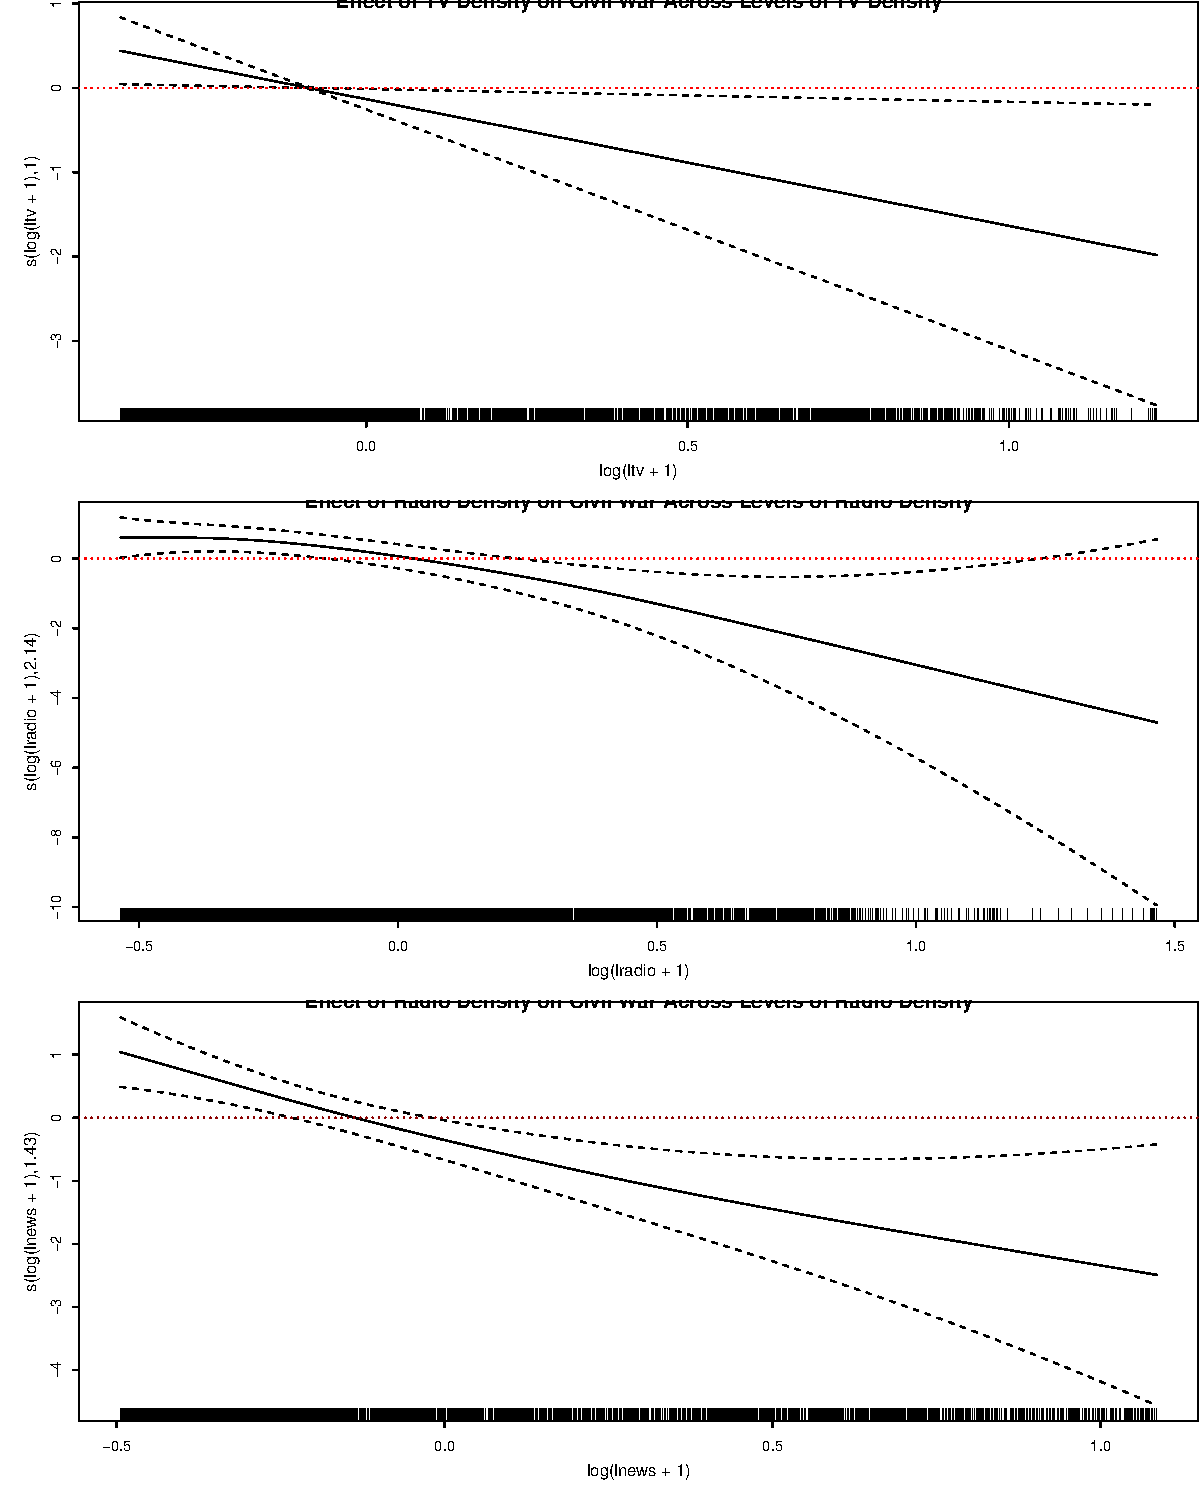
\includegraphics{media_civil_war_files/figure-markdown/disaggregated-nonlinear.pdf}

\begin{figure}
\caption{The non-linear effects of disaggregated media technologies on civil war onset}  
\end{figure}

\pagebreak   

\section{References}\label{references}

\setlength{\parindent}{-0.2in} \setlength{\leftskip}{0.2in}
\setlength{\parskip}{8pt} \vspace*{-0.2in} \noindent

Anderson, Benedict. 1983. \emph{Imagined Communities: Reflections on the
Origin and Spread of Nationalism}. London: Verso.

Bolt, J. 2013. ``The First Update of the Maddison Project; Re-Estimating
Growth Before 1820.'' \emph{Maddison Project Working Paper} 4.

Brass, Paul R. 1997. \emph{Theft of an Idol: Text and Context in the
Representation of Collective Violence}. Princeton: Princeton University
Press.

Chwe, Michael Suk-Young. 1998. ``Culture, Circles, and Commercials:
Publicity, Common Knowledge, and Social Coordination.''
\emph{Rationality and Society} 10(1): 47--75.

---------. 2001. \emph{Rational Ritual: Culture, Coordination, and
Common Knowledge}. Princeton: Princeton University Press.

Correlates of War Project. 2011. ``State System Membership List,
V2011.'' \url{http://correlatesofwar.org}.

Des Forges, Allison. 1999. \emph{Leave None to Tell the Story: Genocide
in Rwanda}. New York: Human Rights Watch.

Deutsch, Karl W. 1953. \emph{Nationalism and Social Communication: an
Inquiry into the Foundations of Nationality}. New York: Technology
Press.

Fearon, James D, and David D Laitin. 2003. ``Ethnicity, Insurgency, and
Civil War.'' \emph{American Political Science Review} 75-90(01): 75.

Fox, John. 2002. \emph{An R and S-Plus Companion to Applied Regression}.
Thousand Oaks, CA: Sage.

Fr{ö}lich, Markus. 2006. ``Non-Parametric Regression for Binary
Dependent Variables.'' \emph{Econometrics Journal} 9(3): 511--40.

Gagnon Jr, V.P. 1994. ``Ethnic Nationalism and International Conflict:
The Case of Serbia.'' \emph{International Security} 19(3): 130.

Gelman, Andrew. 2008. ``Scaling Regression Inputs by Dividing by Two
Standard Deviations.'' \emph{Statistics in Medicine} 27(15): 2865--73.

Hintze, Jerry L, and Ray D Nelson. 1998. ``Violin Plots: A Box
Plot-Density Trace Synergism.'' \emph{The American Statistician} 52(2):
181--84.

Hubbard, Ben, and Hwaida Saad. 2014. ``Pro-Hezbollah Song Opens Musical
Front in Civil War Over Syria.'' \emph{The New York Times}.
\url{http://nyti.ms/1g1w8Iy}.

Im, Kyung So, M Hashem Pesaran, and Yongcheol Shin. 2003. ``Testing for
Unit Roots in Heterogeneous Panels.'' \emph{Journal of Econometrics}
115(1): 53--74.

Imai, Kosuke, Gary King, and Olivia Lau. 2009. ``Zelig: Everyone's
Statistical Software.''

Kastellec, Jonathan P, and Eduardo L Leoni. 2007. ``Using Graphs Instead
of Tables in Political Science.'' \emph{Perspectives on Politics} 5(04):
755--71.

Kellow, C.L., and H.L. Steeves. 1998. ``The Role of Radio in the Rwandan
Genocide.'' \emph{Journal of Communication} 48(3): 107--28.

Keohane, Robert O, and Joseph S Nye. 1998. ``Power and Interdependence
in the Information Age.'' \emph{Foreign Affairs} 77(5): 81.

Kern, Holger Lutz, and Jens Hainmueller. 2009. ``Opium for the Masses:
How Foreign Media Can Stabilize Authoritarian Regimes.'' \emph{Political
Analysis} 17(4): 377--99.

King, Gary, and Langche Zeng. 2001. ``Logistic Regression in Rare Events
Data.'' \emph{Political Analysis} 9(2): 137--63.

King, Ging, Robert O Keohane, and Sidney Verba. 1994. \emph{Designing
Social Inquiry: Scientific Inference in Qualitative Research}.
Princeton: Princeton University Press.

Kirkpatrick, David D. 2011. ``Hopes for a Qaddafi Exit, and Worries of
What Comes Next.'' \emph{The New York Times}.
\url{http://www.nytimes.com/2011/03/22/world/africa/22tripoli.html?pagewanted=all\&_r=0}.

Levin, Andrew, Chien-Fu Lin, and Chia-Shang James Chu. 2002. ``Unit Root
Tests in Panel Data: Asymptotic and Finite-Sample Properties.''
\emph{Journal of Econometrics} 108(1): 1--24.

Lyall, Jason, and Allan Dafoe. 2015. ``From Cell Phones to Conflict?
Reflections on the Emerging ICT-Political Conflict Research Agenda.''
\emph{Journal of Peace Research}.

Metzl, Jamie Frederic. 1997. ``Rwandan Genocide and the International
Law of Radio Jamming.'' \emph{The American Journal of International Law}
91(4): 628.

Mutz, Diana C. 1998. \emph{Impersonal Influence: How Perceptions of Mass
Collectives Affect Political Attitudes}. Cambridge: Cambridge University
Press.

Nye, Joseph S. 1990. ``Soft Power'' \emph{Foreign Policy} (80): 153--71.

---------. 2004. \emph{Soft Power: The Means to Success in World
Politics}. New York: Public Affairs.

Paluck, Elizabeth Levy. 2009. ``Reducing Intergroup Prejudice and
Conflict Using the Media: A Field Experiment in Rwanda.'' \emph{Journal
of Personality and Social Psychology} 96(3): 574--87.

``Roads Sealed as Yugoslav Unrest Mounts.'' 1990. \emph{The New York
Times}.
\url{http://www.nytimes.com/1990/08/19/world/roads-sealed-as-yugoslav-unrest-mounts.html}.

Sambanis, N. 2004. ``What Is Civil War?: Conceptual and Empirical
Complexities of an Operational Definition.'' \emph{Journal of Conflict
Resolution} 48(6): 814--58.

Simons, Marlise. 2002. ``Trial Centers on Role of Press During Rwanda
Massacre.'' \emph{The New York Times}. \url{http://nyti.ms/1DQPT66}.

Straus, Scott. 2007. ``What Is the Relationship Between Hate Radio and
Violence? Rethinking Rwanda's Radio Machete.'' \emph{Politics \&
Society} 35(4): 609--37.

Tambiah, Stanley J. 1996. \emph{Leveling Crowds: Ethnonationalist
Conflicts and Collective Violence in South Asia}. Berkeley: University
of California Press.

Warren, T Camber. 2014. ``Not by the Sword Alone: Soft Power, Mass
Media, and the Production of State Sovereignty.'' \emph{International
Organization} 68(01): 111--41.

Wood, S N. 2000. ``Modelling and Smoothing Parameter Estimation with
Multiple Quadratic Penalties.'' \emph{Journal of the Royal Statistical
Society B} 62(2): 413--28.


\end{document}